\section{Preliminary Project}
\label{sec:preliminary_project}
The preliminary project section provides an overview of the hydrography management system project for the Province of Belluno. It covers various aspects, including goals, system functions, databases, technological components, project guidelines, operational aspects, risk management, benefits evaluation, and cost evaluation. This section serves as a comprehensive summary of the project, outlining its objectives, system functionalities, database structure, technical components, implementation guidelines, and assessment of potential benefits and costs. It provides a holistic view of the project's scope and sets the foundation for its successful execution and management.

\subsection{Goals}
The goals of the hydrography management system project for the Province of Belluno are defined to ensure the successful development, implementation, and utilization of the system. These goals provide a clear direction for our project team and serve as measurable outcomes to evaluate the project's success. The goals can be categorized into two key areas: overarching goals and intermediate goals.
\subsubsection{Overarching Goals}

\begin{itemize}
    \item \textbf{Develop a comprehensive hydrography management system}: The primary goal of the project is to design, develop, and implement a comprehensive hydrography management system tailored to the specific requirements of the Province of Belluno. The system will enable efficient management of water resources, including the documentation of water bodies, tracking of intakes, monitoring of water conditions, and citizen alert management;
    \item \textbf{Ensure user-friendly access and compatibility}: The system should provide a user-friendly interface accessible through popular web browsers such as Explorer, Chrome, and Firefox. Additionally, it should support specific functionality through customized desktop GIS tools when necessary. Compatibility and ease of use are essential to ensure widespread adoption and efficient utilization by technical offices, internal technicians, and citizens;
    \item \textbf{Adhere to relevant standards and regulations}: The system must comply with applicable hydrography management standards and regulations. It should ensure accurate data representation, support data interchangeability using standard formats, and promote interoperability with other systems in the hydrography management domain.
\end{itemize}

\subsubsection{Intermediate Goals}
\begin{itemize}
    \item Enable efficient data management, so to develop functionality for importing and exporting data in shape format and other standard formats, allowing seamless integration with existing datasets and data exchange with external systems. Implement mechanisms for network updates, both in terms of geometric elements and attribute data, ensuring the historicization of changes to track the evolution of the hydrography network;
    \item Implement advanced querying and visualization capabilities, so to create an advanced interrogation system that combines spatial and alphanumeric filters, empowering users to perform complex queries for retrieving relevant information. Enable the export of query results and provide visualization capabilities for cartography and orthophotos as a background, enhancing data analysis and decision-making processes;
    \item Support intake management, so to develop features to enable the identification and management of intakes, including their positions and attributes. Implement functionality for inserting new intakes, removing abandoned ones, and determining the routes of pollutants released from intakes;
    \item Facilitate water condition monitoring, so to design and implement mechanisms to collect real-time data from water monitoring units strategically located throughout the province. Capture key parameters such as water level, flow, turbidity, temperature, conductivity, pH, redox potential, dissolved oxygen, NH4+, and CL- to enable effective monitoring of water conditions;
    \item Enable maintenance planning and execution, so to develop functionality to support the scheduling and execution recording of periodic maintenance tasks for the monitoring units. Ensure timely and efficient maintenance to maintain accurate and reliable data collection;
    \item Enable data consultation and emergency detection, so to implement features that allow technical offices to carry out combined searches, spatial and attribute-based, as well as historical queries to retrieve relevant data. Develop mechanisms to detect and notify relevant personnel of potential emergencies through email notifications triggered by abnormal parameter values;
    \item Establish citizen reporting and transparency. The aim is to create a dedicated portal to publish daily water quality analysis results and promote transparent governance. Develop a reporting system for citizens to anonymously report pollutants with photo attachments and geographical location indications. Implement automatic filtering and relevance scoring of reports to streamline manual processing and associate alerts with relevant monitoring units and previous alerts.
\end{itemize}


\subsection{Technological components}
Whenever talking about a system in the IT field it is implicit that different technological components (being them more or less interconnected) are required. In the case of the proposal for a Hydrography Management System, meeting the requirements of the customer, two different systems has top be developed: a desktop GIS system and a web GIS system, that are introduced in the following subsections and deeply explored in a dedicated paragraph. After that, software and hardware requirements need to be exploited.

\subsubsection{Database}
We can consider the database of the system the glue of all the other technological components. Furthermore, the customer already has in his IT sector a PosgreSQL database, that adapts prefectly to the system we want to develop, thanks to his extension \textit{PostGIS} that is suitable for managing spatial ang geographical data. Hence, this component will be used as the base for the developing of our application.
\subsubsection{Desktop GIS system}
Since is accepted that some of the funtional requirements can be met through a desktop GIS application, and to stay adherent to the non-functional requirement of using FOSS components, the solution found is to develop specific plugins for the \textit{OpenJUMP} desktop application, making use of the \textit{Java™ JTS library}; the plugins built for the system will be packed together with the application and delivered to the customer. Technical support for the installation of the desktop system on customer terminals will be provided.
\subsubsection{Web GIS system}
The core of the system will be the web application: since it has to deliver to the user GIS capabilities, many components need to be integrated:
\begin{itemize}
    \item Frontend map management: it is necessary to provide to the users the possibility to use maps through the web app. For this, the OpenLayer JavaScript plugin will be used;
    \item Background map: it is necessary to display in this plugin a background map of the province: to meet this requirement, OpenStreetMap maps will be used;
    \item Backend spatial data delivery: it is necessary to deliver to the user (and to display over the OpenStreetMap) the spatial data that the Veneto Region has at disposal: for this, a dedicated Geoserver instance is necessary;
    \item Frontend implementation: parts of the web application shall be used also from the provincial citizens even on the go from mobile devices. In an optic of usability of the system with any device it is necessary of a full responsiveness of the system over any kind of terminal (smartphones, tablets, etc.) and to better integrate with other public IT systems, the \textit{Bootstrap Italia} template is our implementational choice.
\end{itemize}

\subsubsection{Hardware requirements}
To support the functioning of the web application also from the exterior of the provincial organization, because of the active citizenship policy, but also to facilitate eventual and future possibilities of smart working activities of the provincial employees, a concrete possibility is the one of setting up a virtual private server hosted on the cloud: this possibility can be delivered both from a provate hosting company, with a cost that has to be kept in consideration, or by the availability of some italian server infrastructure, if any.
The fact that the customer already owns a PostgreSQL database in their servers, can suggest to use them as hosting machines also for the system, but this can led to security problems since can be that the machines are used also for other purposes, and the data traffic coming from the new system can cause slowdowns of the machine or worse, of the provincial office network. A solution to this can be to keep the data on the legacy database and tunnel the traffic between the new private server and the native machine whenever interactions with database are necessary, or to replicate the data we are interested on on a new instance of PostgreSQL running on the dedicate new private server.

\subsubsection{Software requirements}
Many softwares needs to be used to set up the system:
\begin{itemize}
    \item \textbf{Operating system}: an operating system has to be installed on the private server: to be stick with the FOSS components requirement, an installation of \textit{Ubuntu server} or \textit{CentOS} can be considered as valid option.
    \item \textbf{Database}: from the considerations derived from previous section, two different approaches can be followed: in case of replication, a fresh installation of PostgreSQL with the PostGIS extension is needed; if this is not considered a valid option, a way to set up a VPN connection between the existing PostgreSQL server and the system' server needs to be setted up.
    \item \textbf{Web server}: a web server capable of delivering web contents, possibly also under SSL certificates, run scripts, and proxy data from other softwares needs to be setted up: for this, the \textit{Apache HTTP server} can be suitable for this requirement.
    \item \textbf{Scripting interpreter}: the logic of the web system will be implemented through \textit{PHP}, a scripting laguage, that needs its interpreter (with the needed extensions) to be setted up properly.
    \item \textbf{Web Map server (WMS)}: a system capable of delivering web maps is needed: for this, \textit{Geoserver} is the best solution available.
    \item \textbf{Web Map server container}: Geoserver is developed as a web application in \textit{Java}. This requires a Java container to run web applications. \textit{Tomcat} is our implementing choice, but a standalone version that includes another container (\textit{Jetty}) can be used.
    \item \textbf{Security}: to better protect the server from malicius trials of intrusion, a firewall software can be installed on the machine. A good approach can be the usage of \textit{iptables}. 
\end{itemize}

\subsubsection{Components Schema}
\begin{figure}[H]
    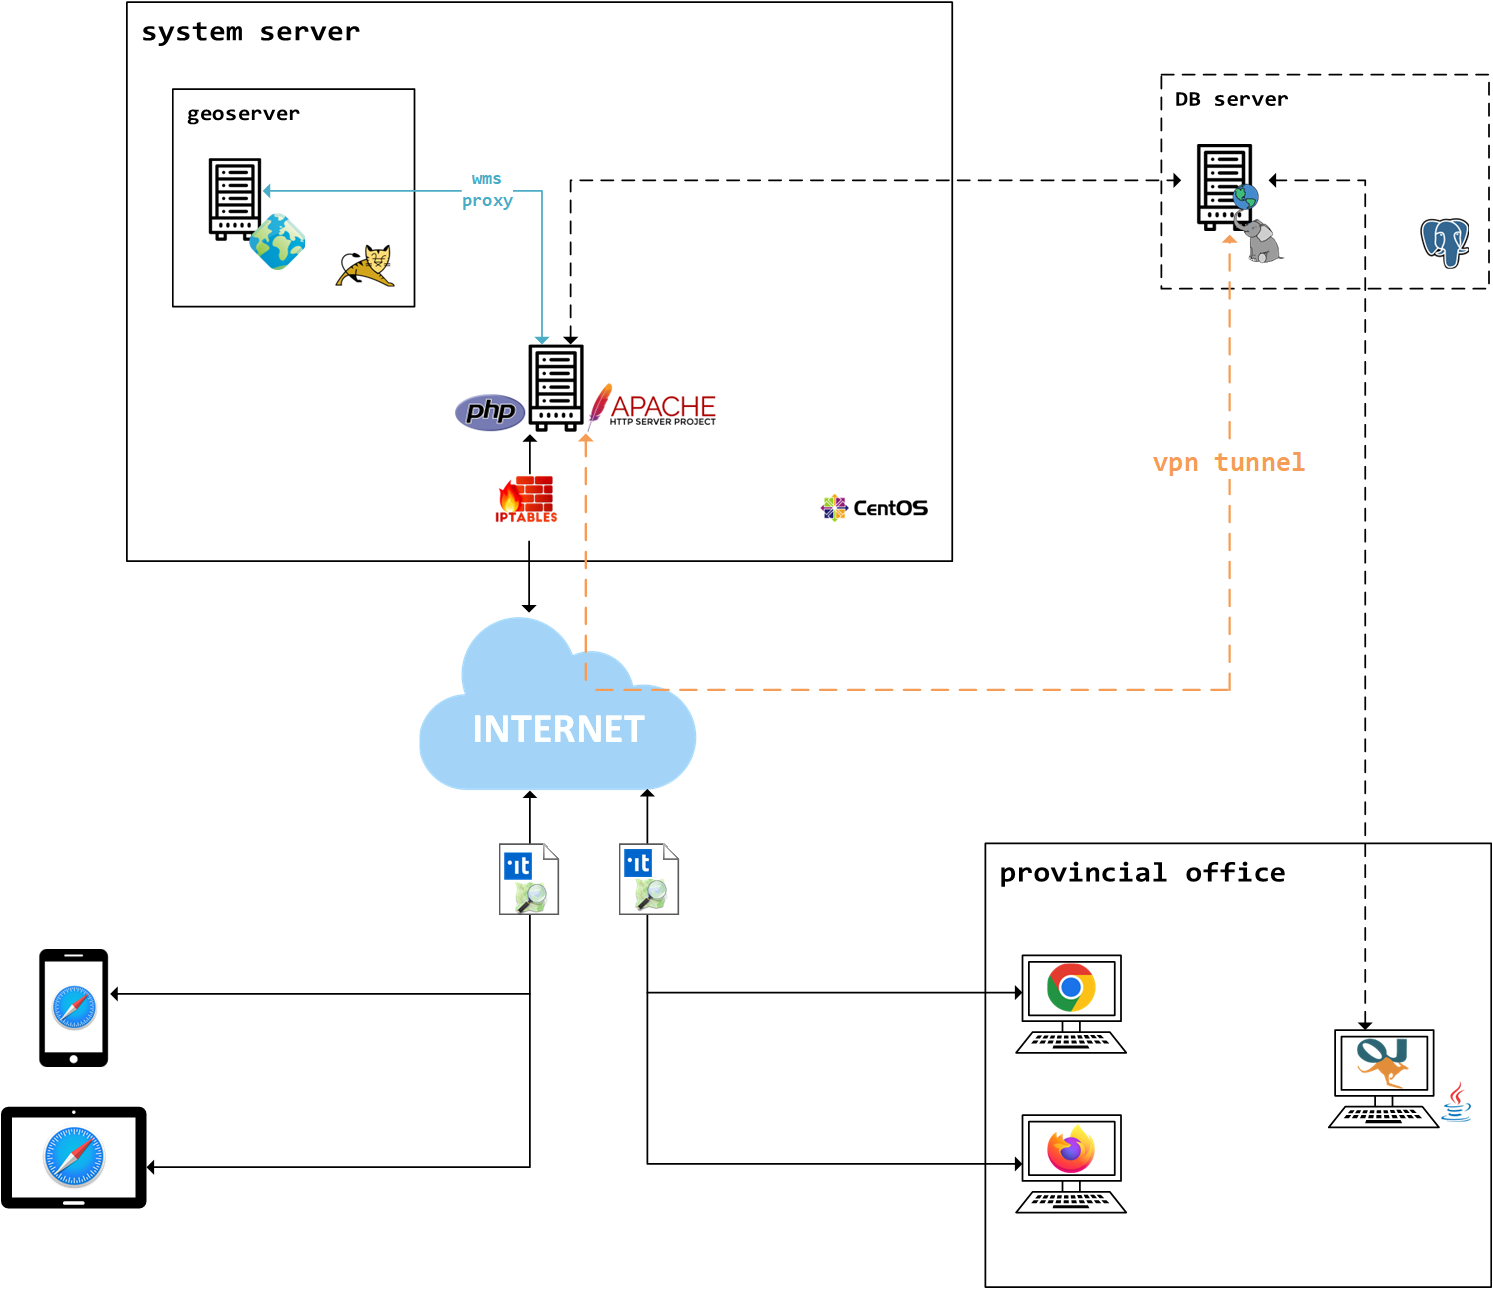
\includegraphics[width=\textwidth]{img/system}
    \caption{Logical schema}
    \label{LogicalSchema}
\end{figure}

\subsection{Functional aspects of the system}
The systems are developed in a way that no specific capabilities are required from the users.
Anyway, here we provide some short explaination of some of the functionalities that we developed as a demo; the usability of the whole application will be based on the same technologies and possible to use in the same way. 
\subsubsection{WebGIS application}
The web application shall be used both from the citizenship side (from mobile devices) and from the provincial technicians, that has to access to the web appllication from a desktop computer.
Starting from the perspective of the citizenship, the functionalities are:
\begin{itemize}
    \vspace{3ex}
    \item \textbf{Home page} \\
    \begin{figure}[H]\centering 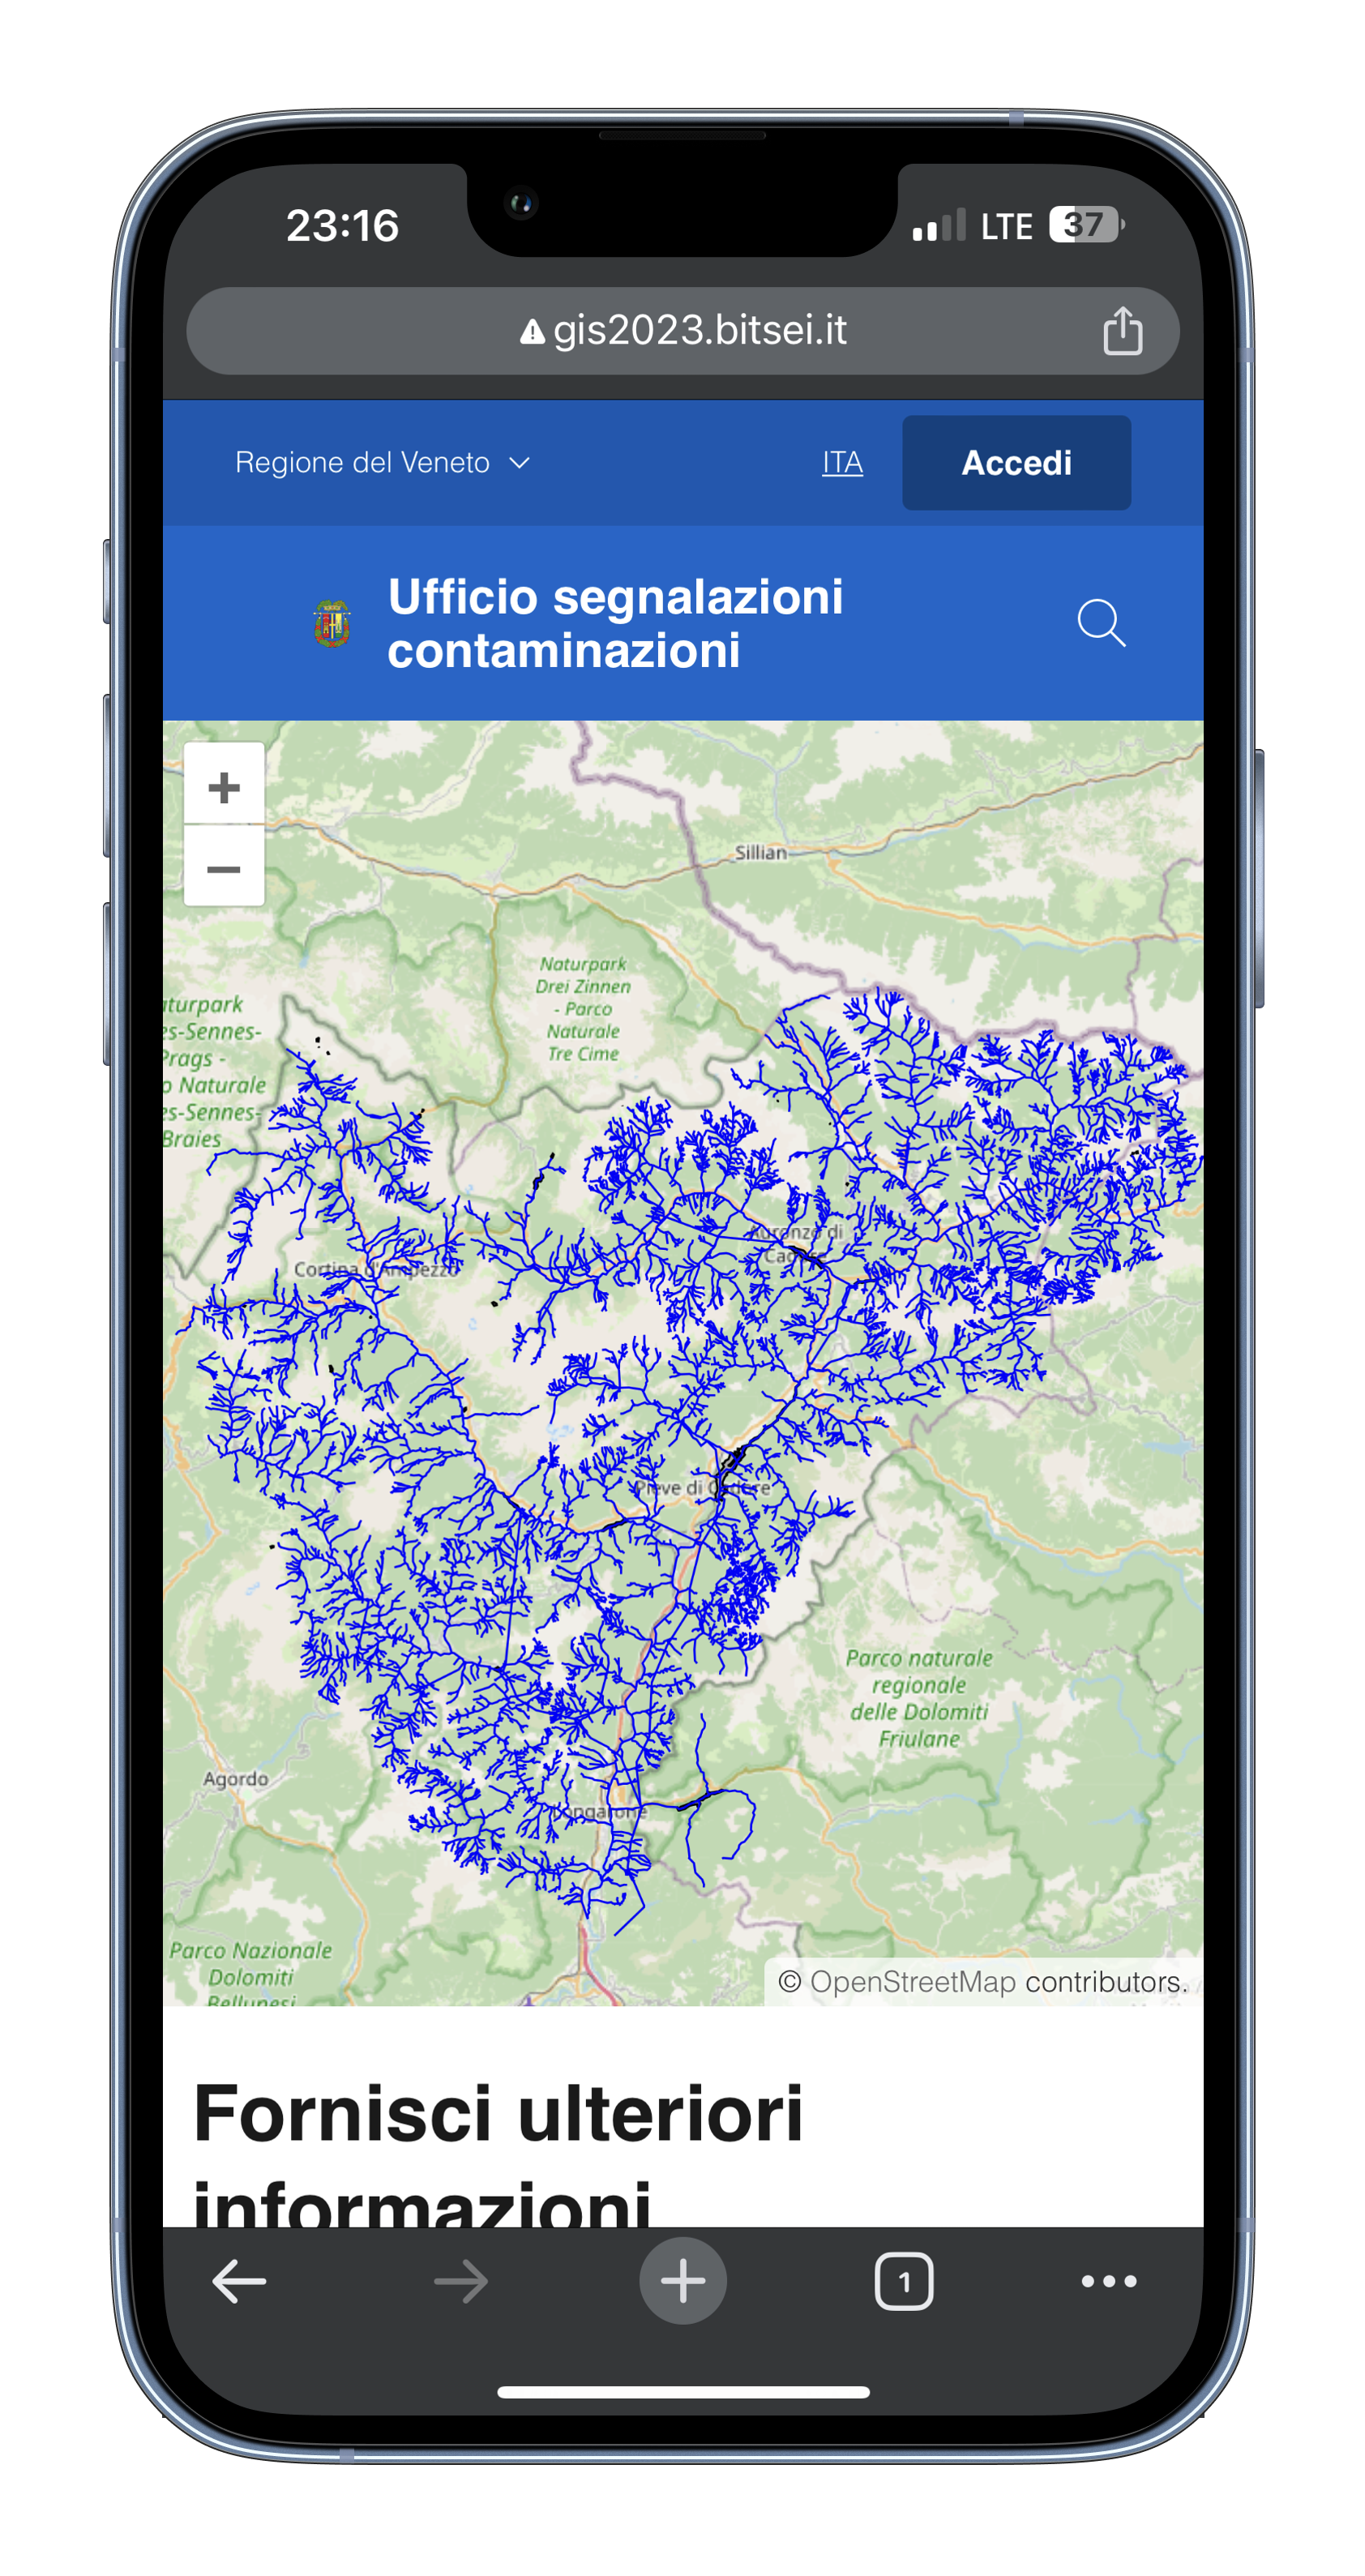
\includegraphics[width=10em]{img/home.png} 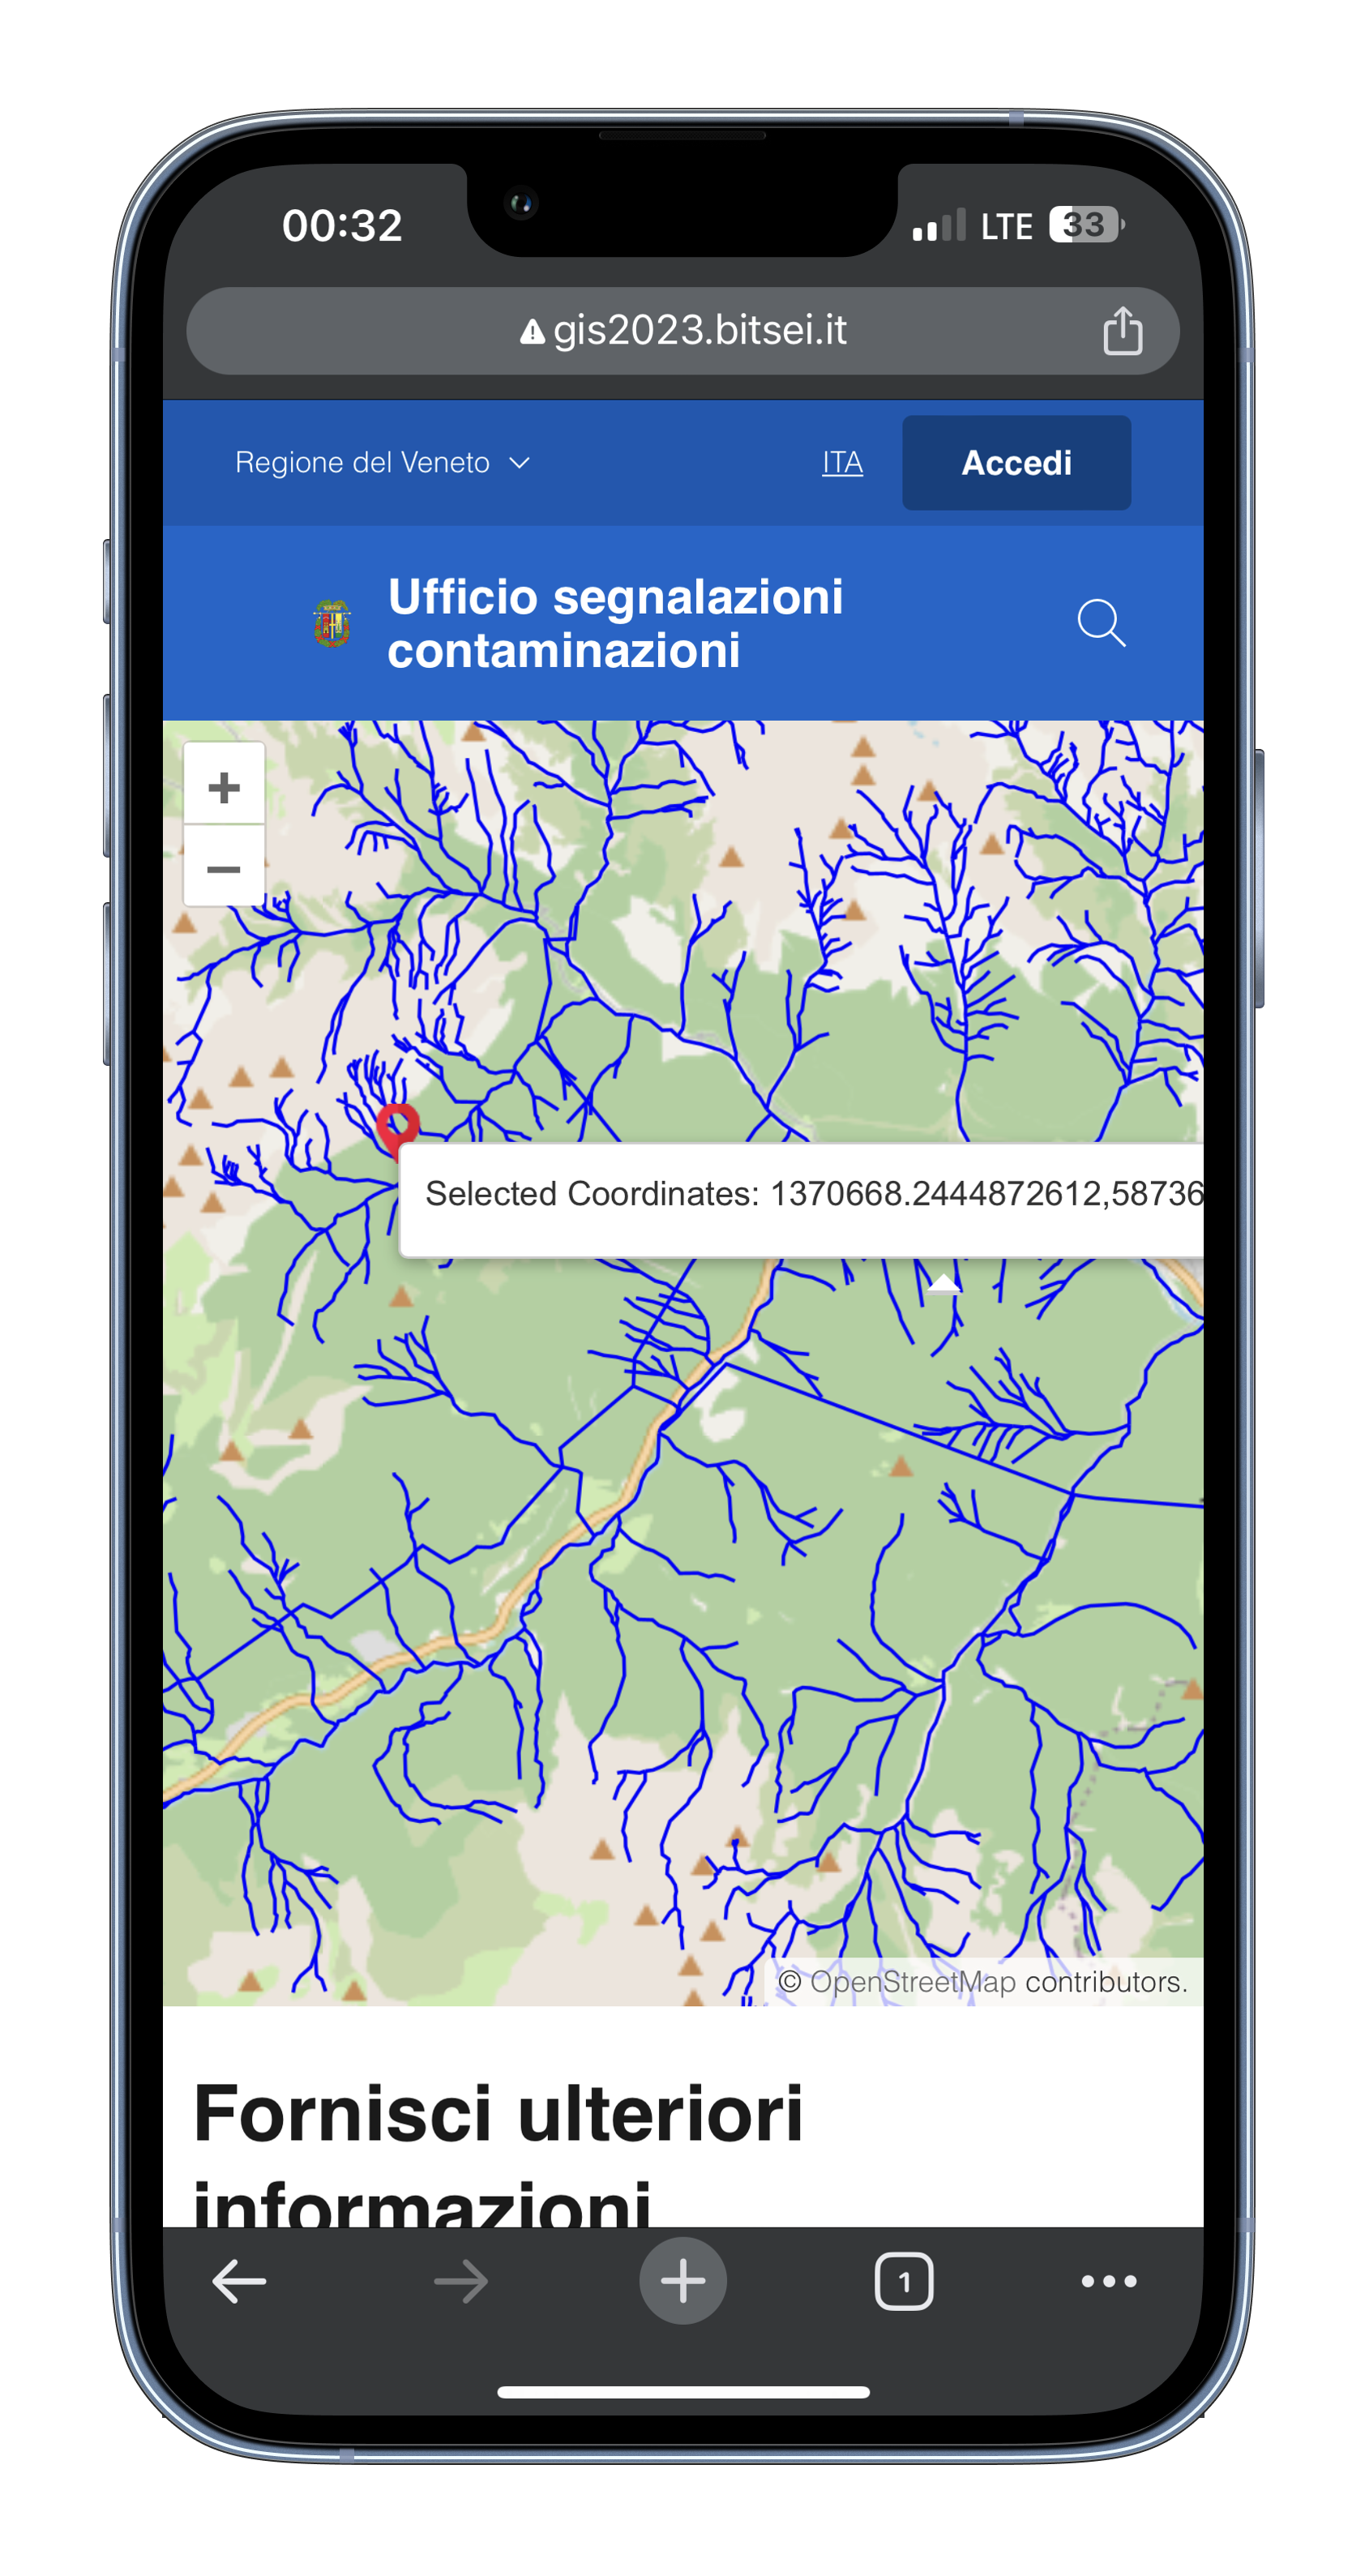
\includegraphics[width=10em]{img/posizione.png} 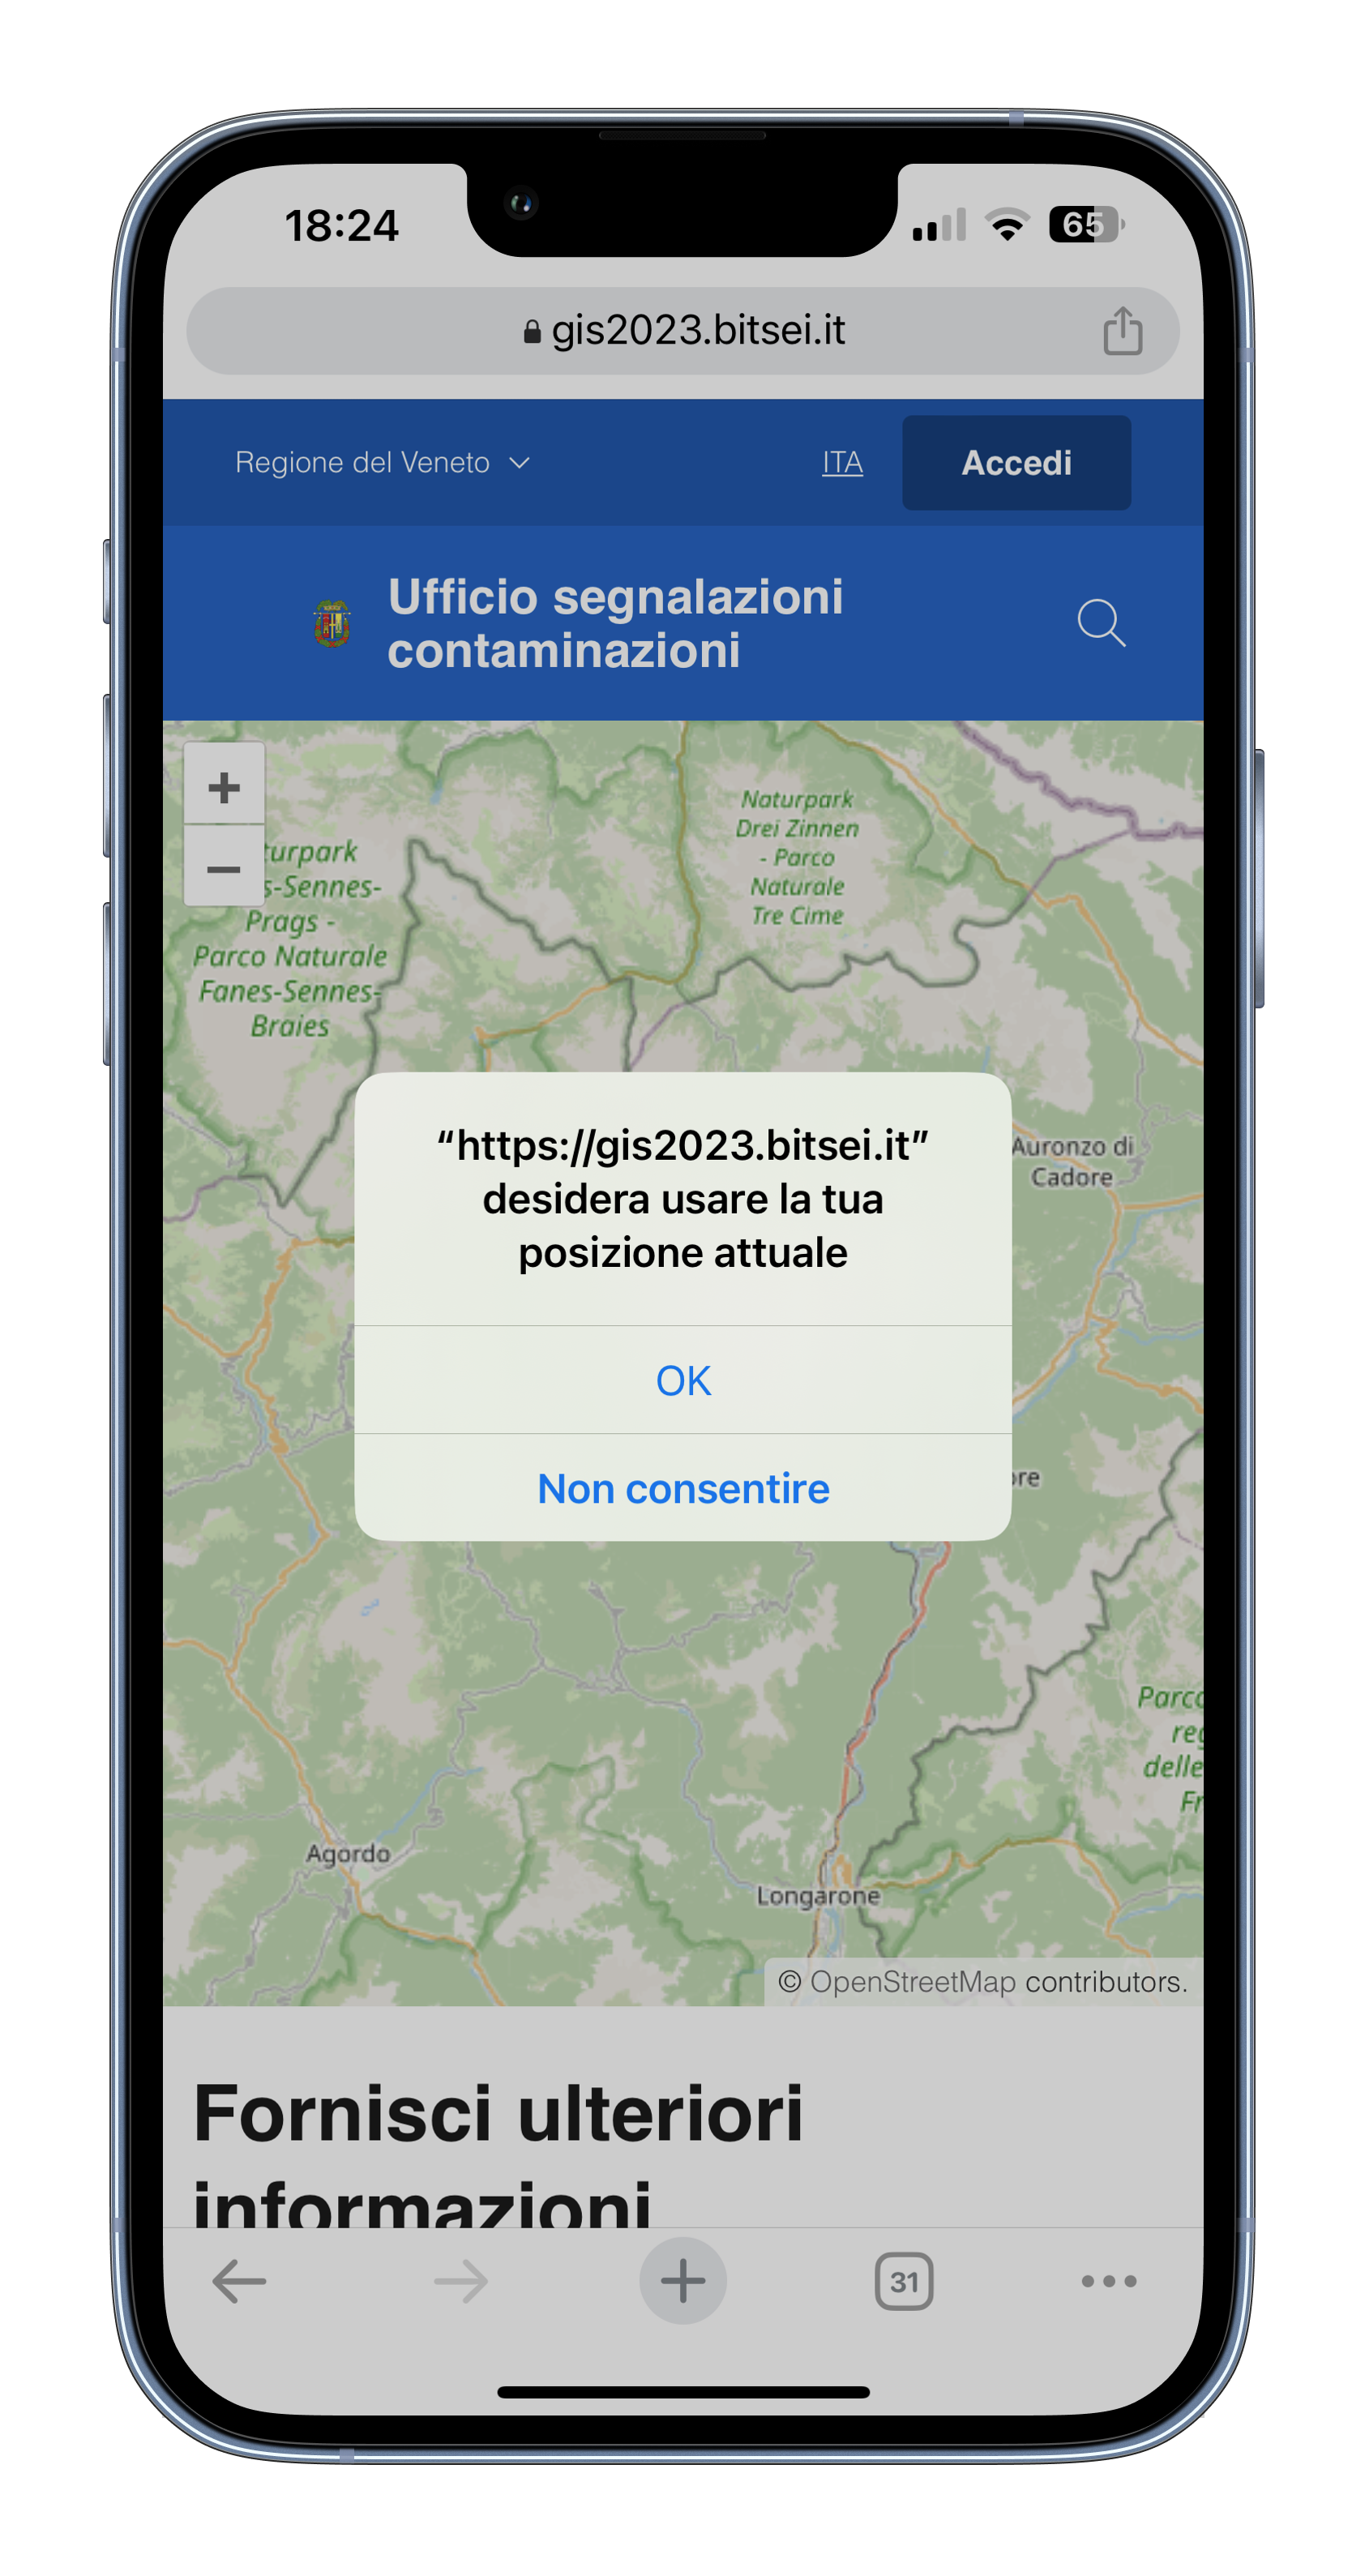
\includegraphics[width=10em]{img/autoposizione.png}  \caption{Smartphone map view} \label{phoneHomepage}\end{figure}
    The page loads showing as a background (under the headings) the map of the province of Belluno; the user can surf the map and select the position by clicking on it; when the page loads the first time, it asks the user to gather the position from the device, without the need of him to choose it manually Fig:[\ref{phoneHomepage}]. \\
    \pagebreak
    \item \textbf{Undergoing form} \\
    \begin{figure}[H] \centering 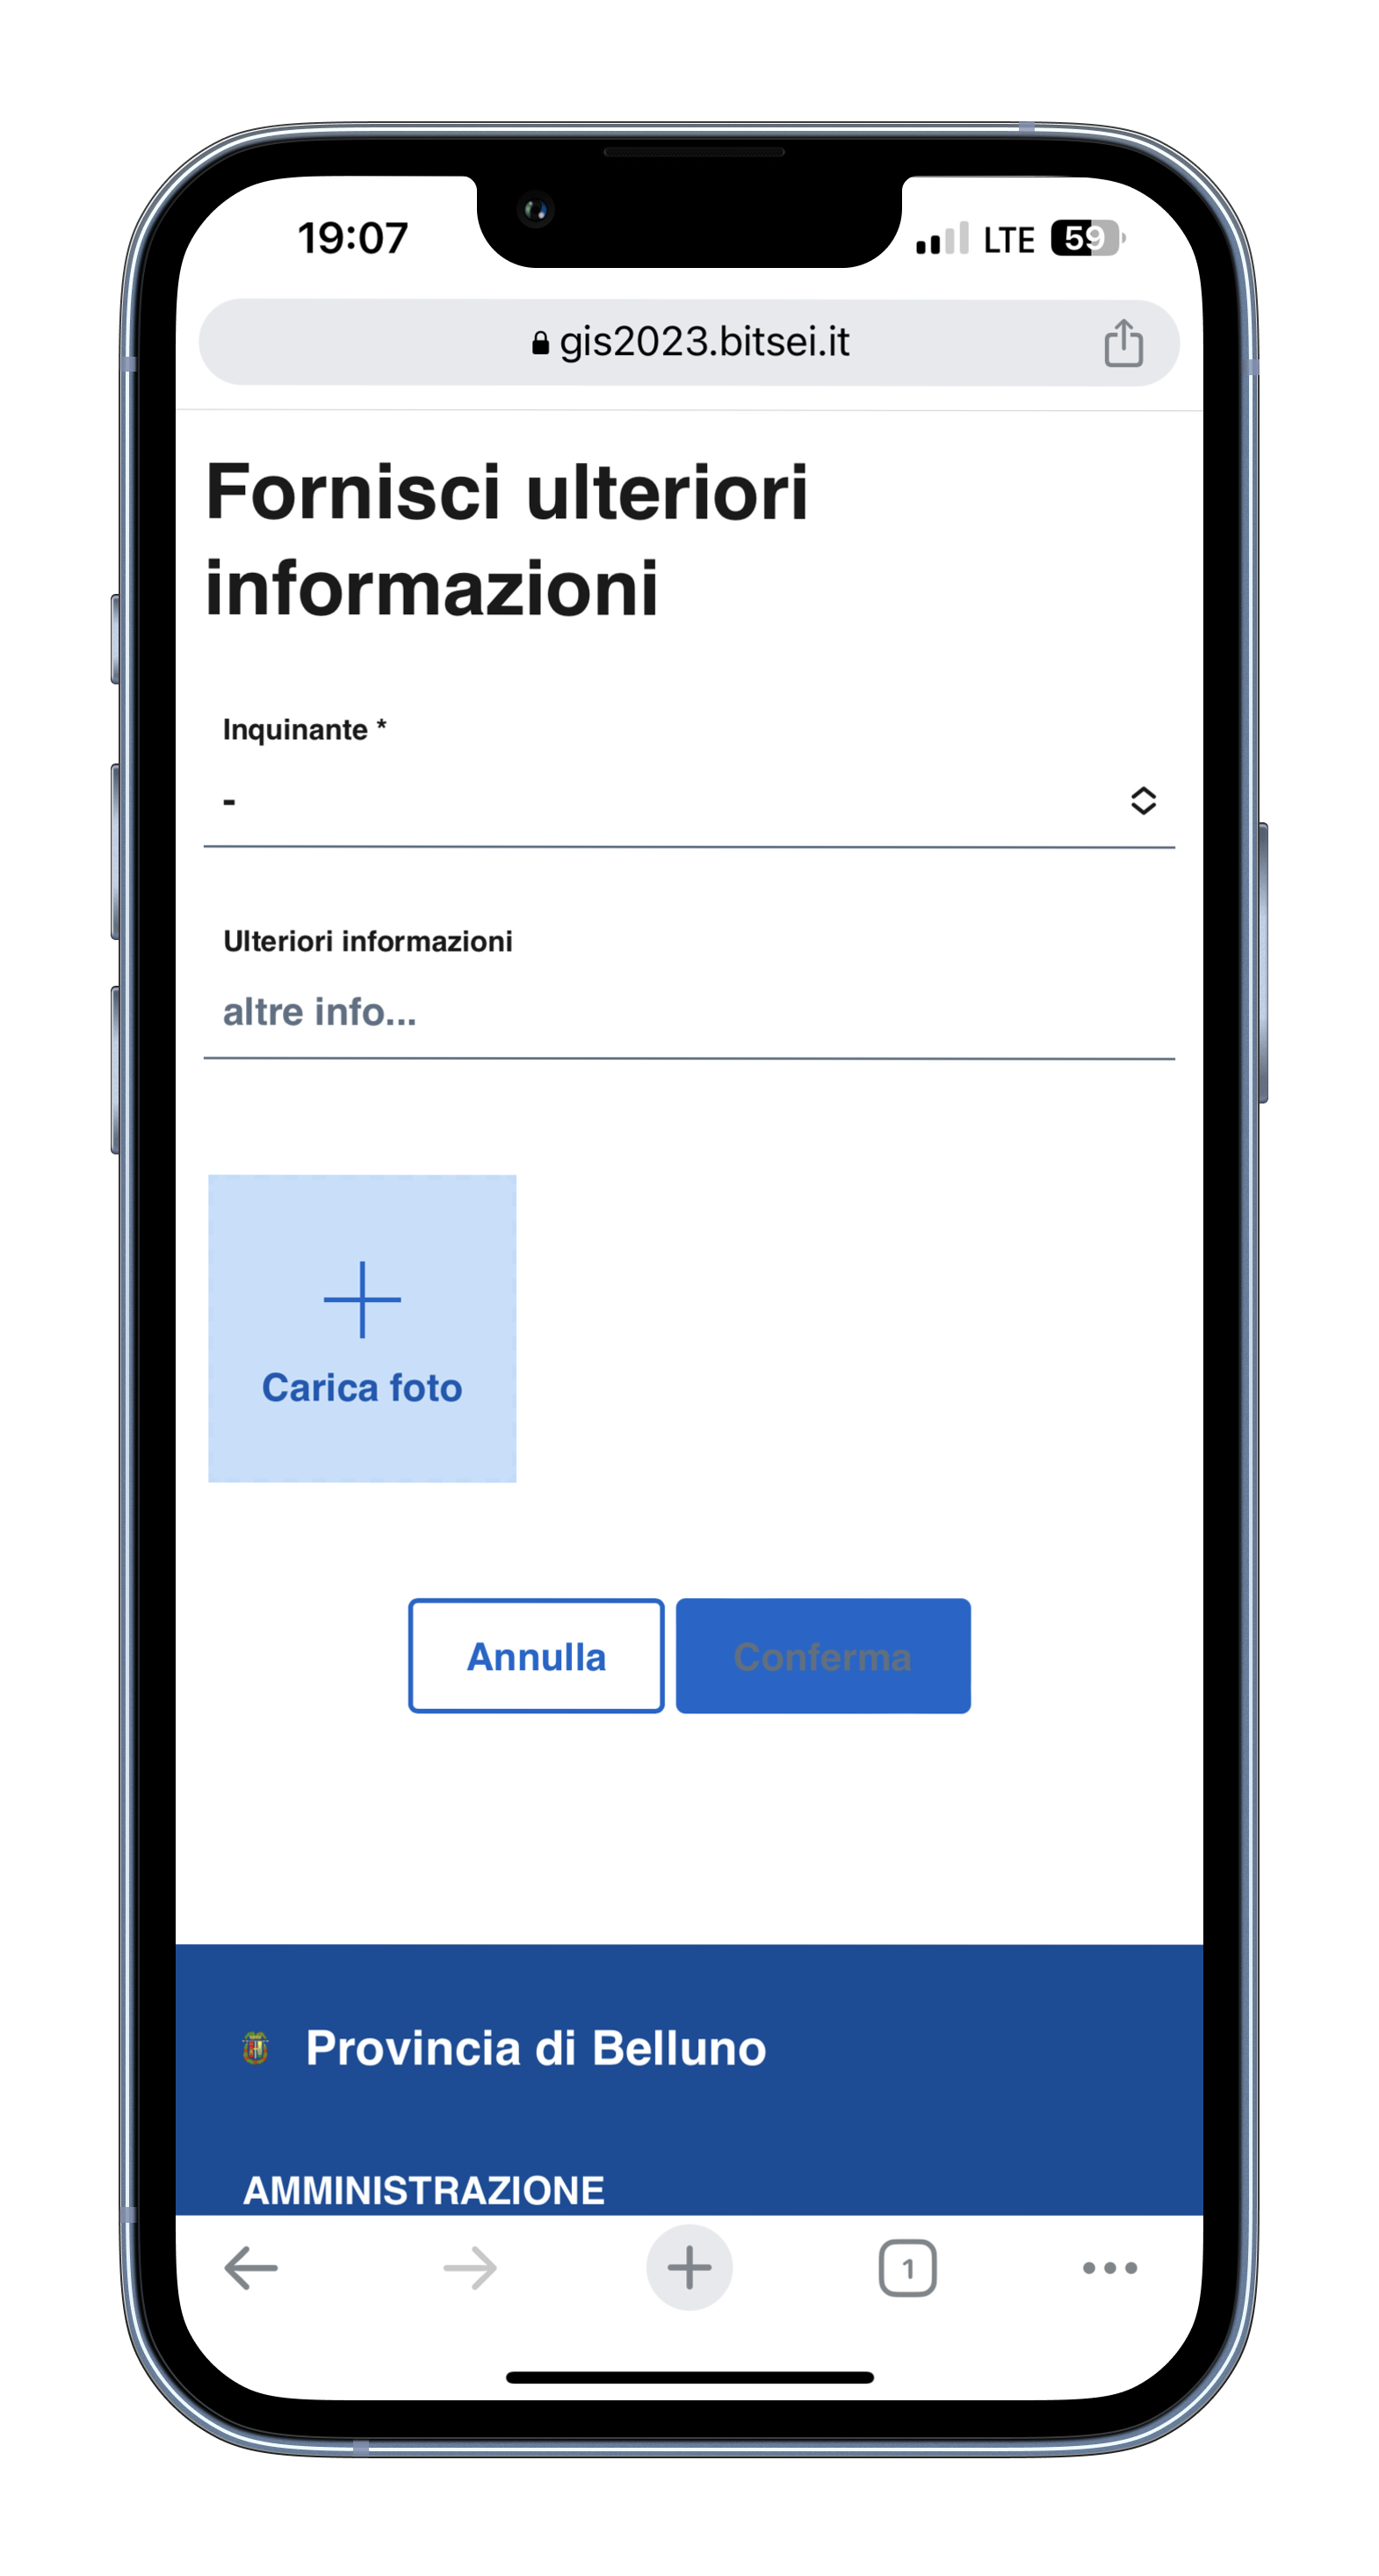
\includegraphics[width=10em]{img/form.png} 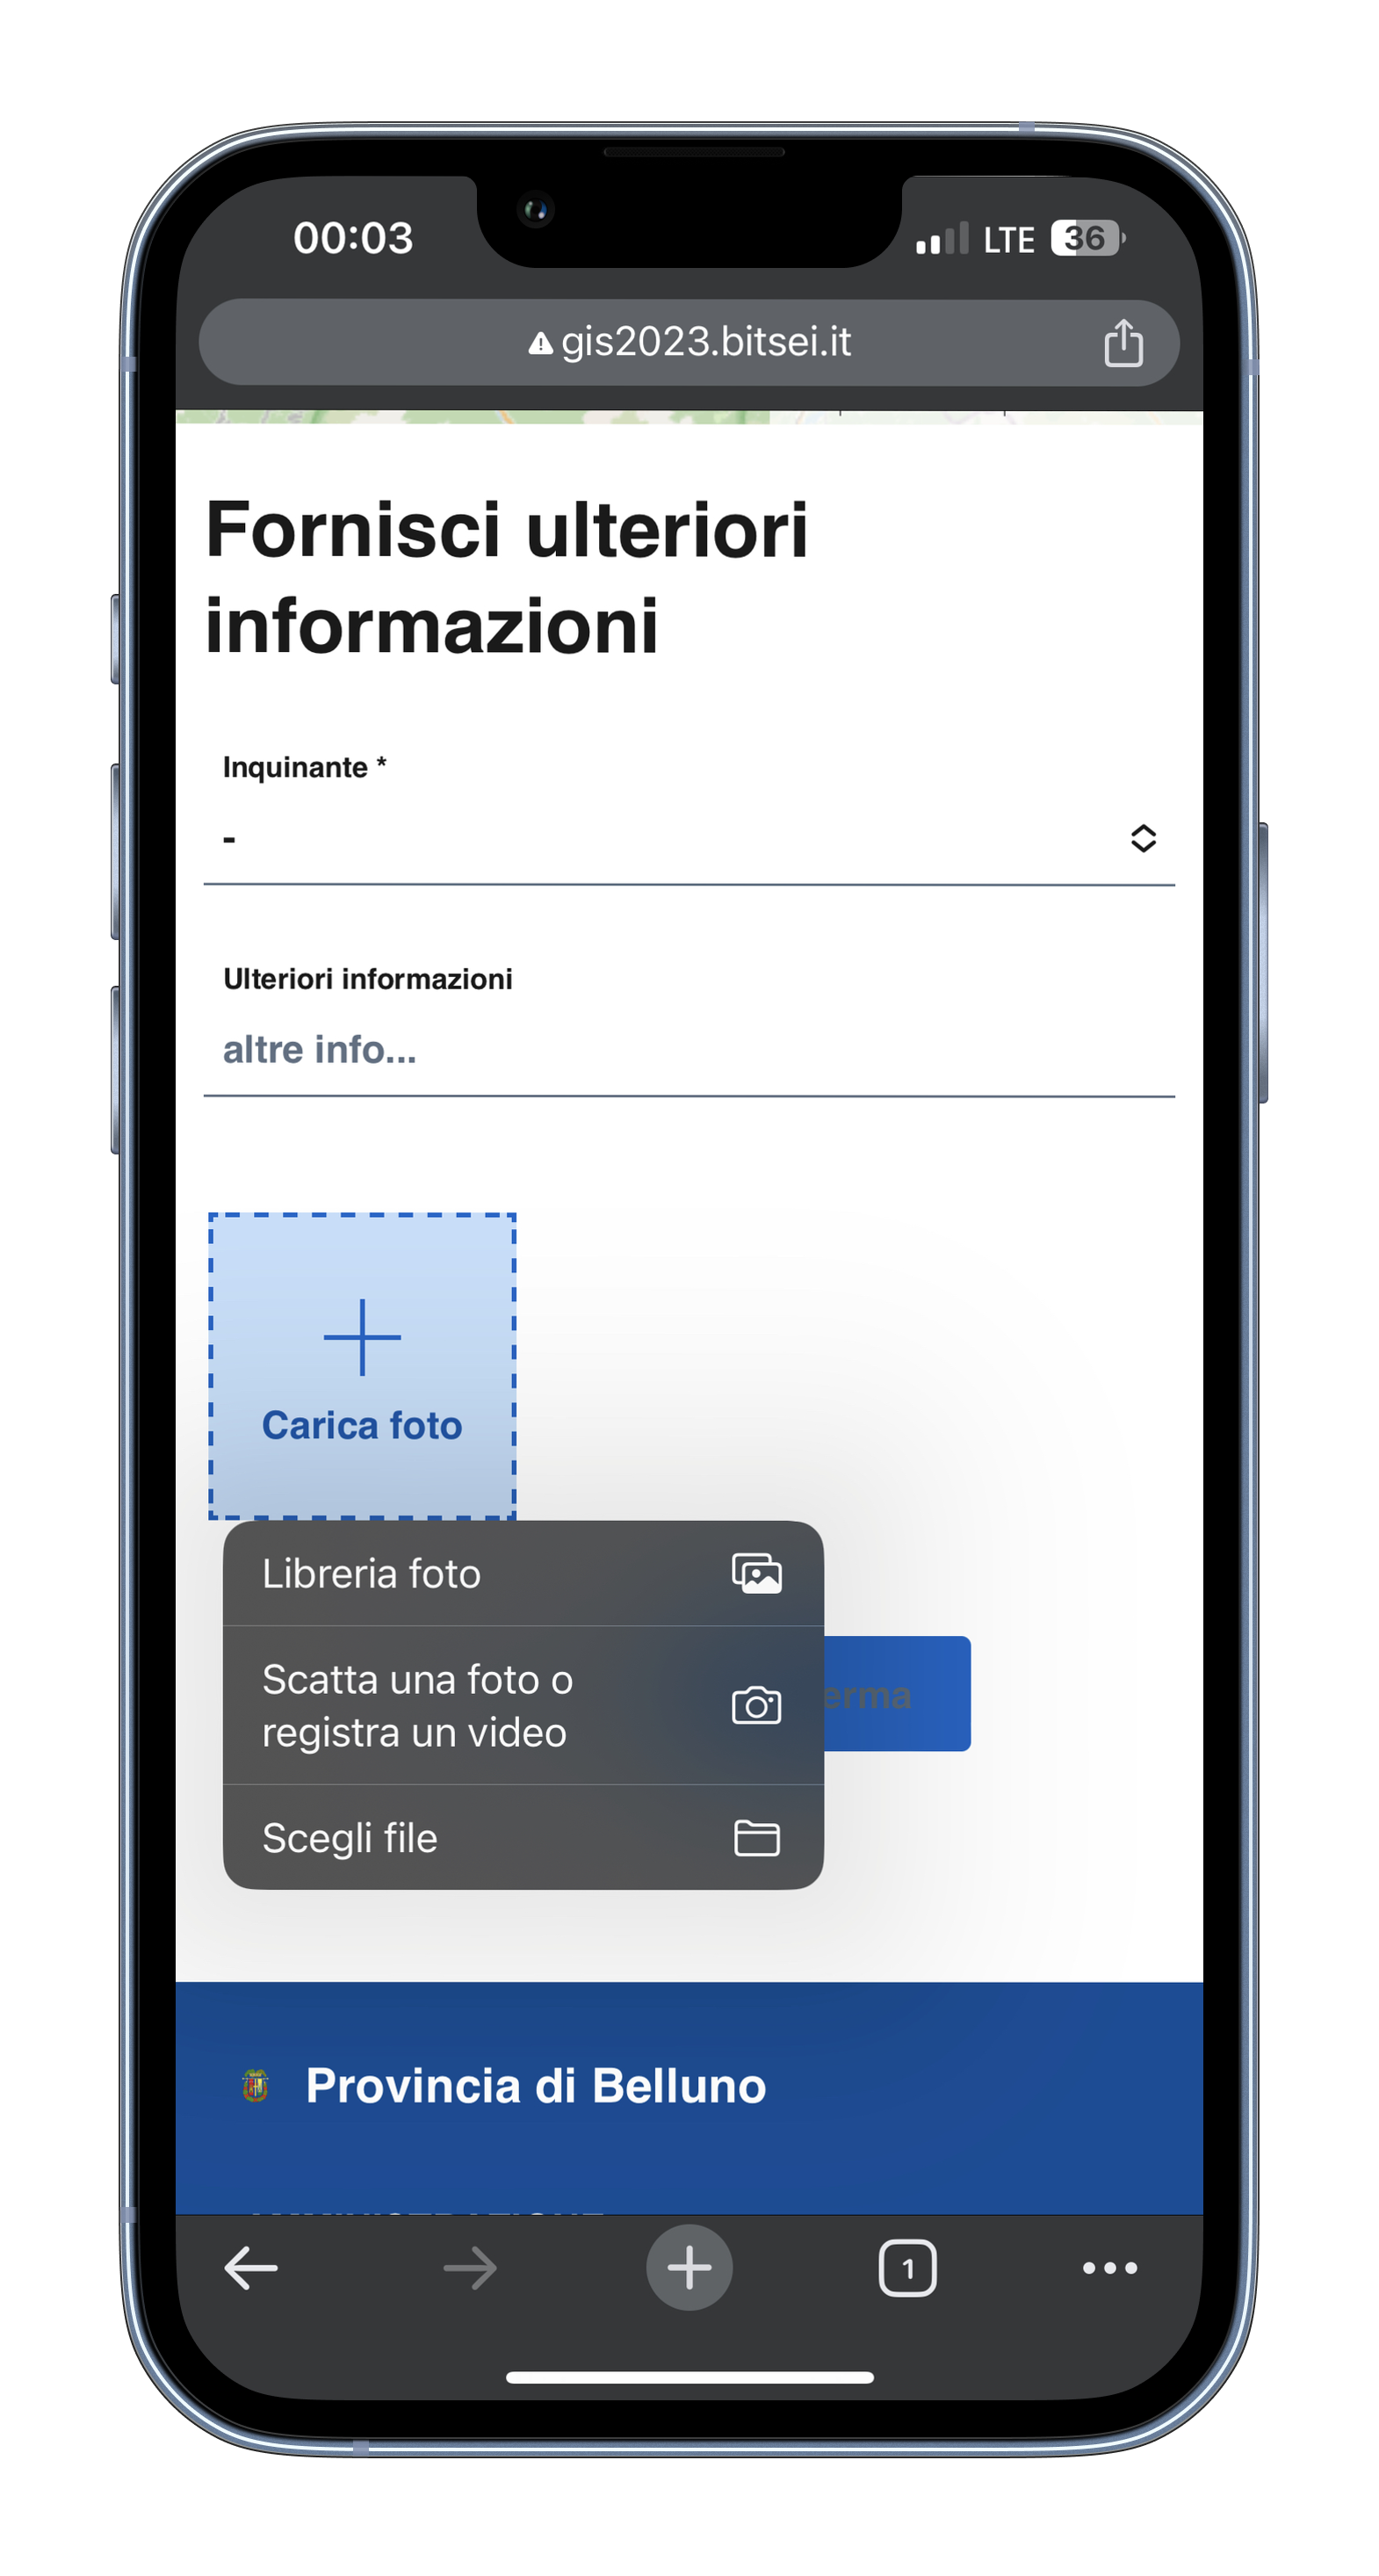
\includegraphics[width=10em]{img/foto.png} \caption{Smartphone view for uploading the the photo} \label{uploafPhoto} \end{figure}
    Under the map the user can fill the remaining form fields: he must select from a dropdown menu the pollutant found; he then can optionally write a description and upload an image, stored in its device or by capturing from the camera Fig:[\ref{uploafPhoto}].
    \vspace{3ex}
    \item \textbf{Usability from a tablet} \\
    All the mentioned functionalities can be also used from a tablet rather than from a smartphones; the responsiveness is still guaranteed Fig[\ref{tablet}]: 
    \begin{figure}[H] \centering \includegraphics[width=22em]{img/tablet.png} \caption{Tablet interface} \label{tablet} \end{figure}
\end{itemize} 
\pagebreak
Switching to the perspective of the provincial technicians we have the following pages and functionalities:
\begin{itemize}
    \item \textbf{Login page} \\
    \begin{figure}[H]\centering 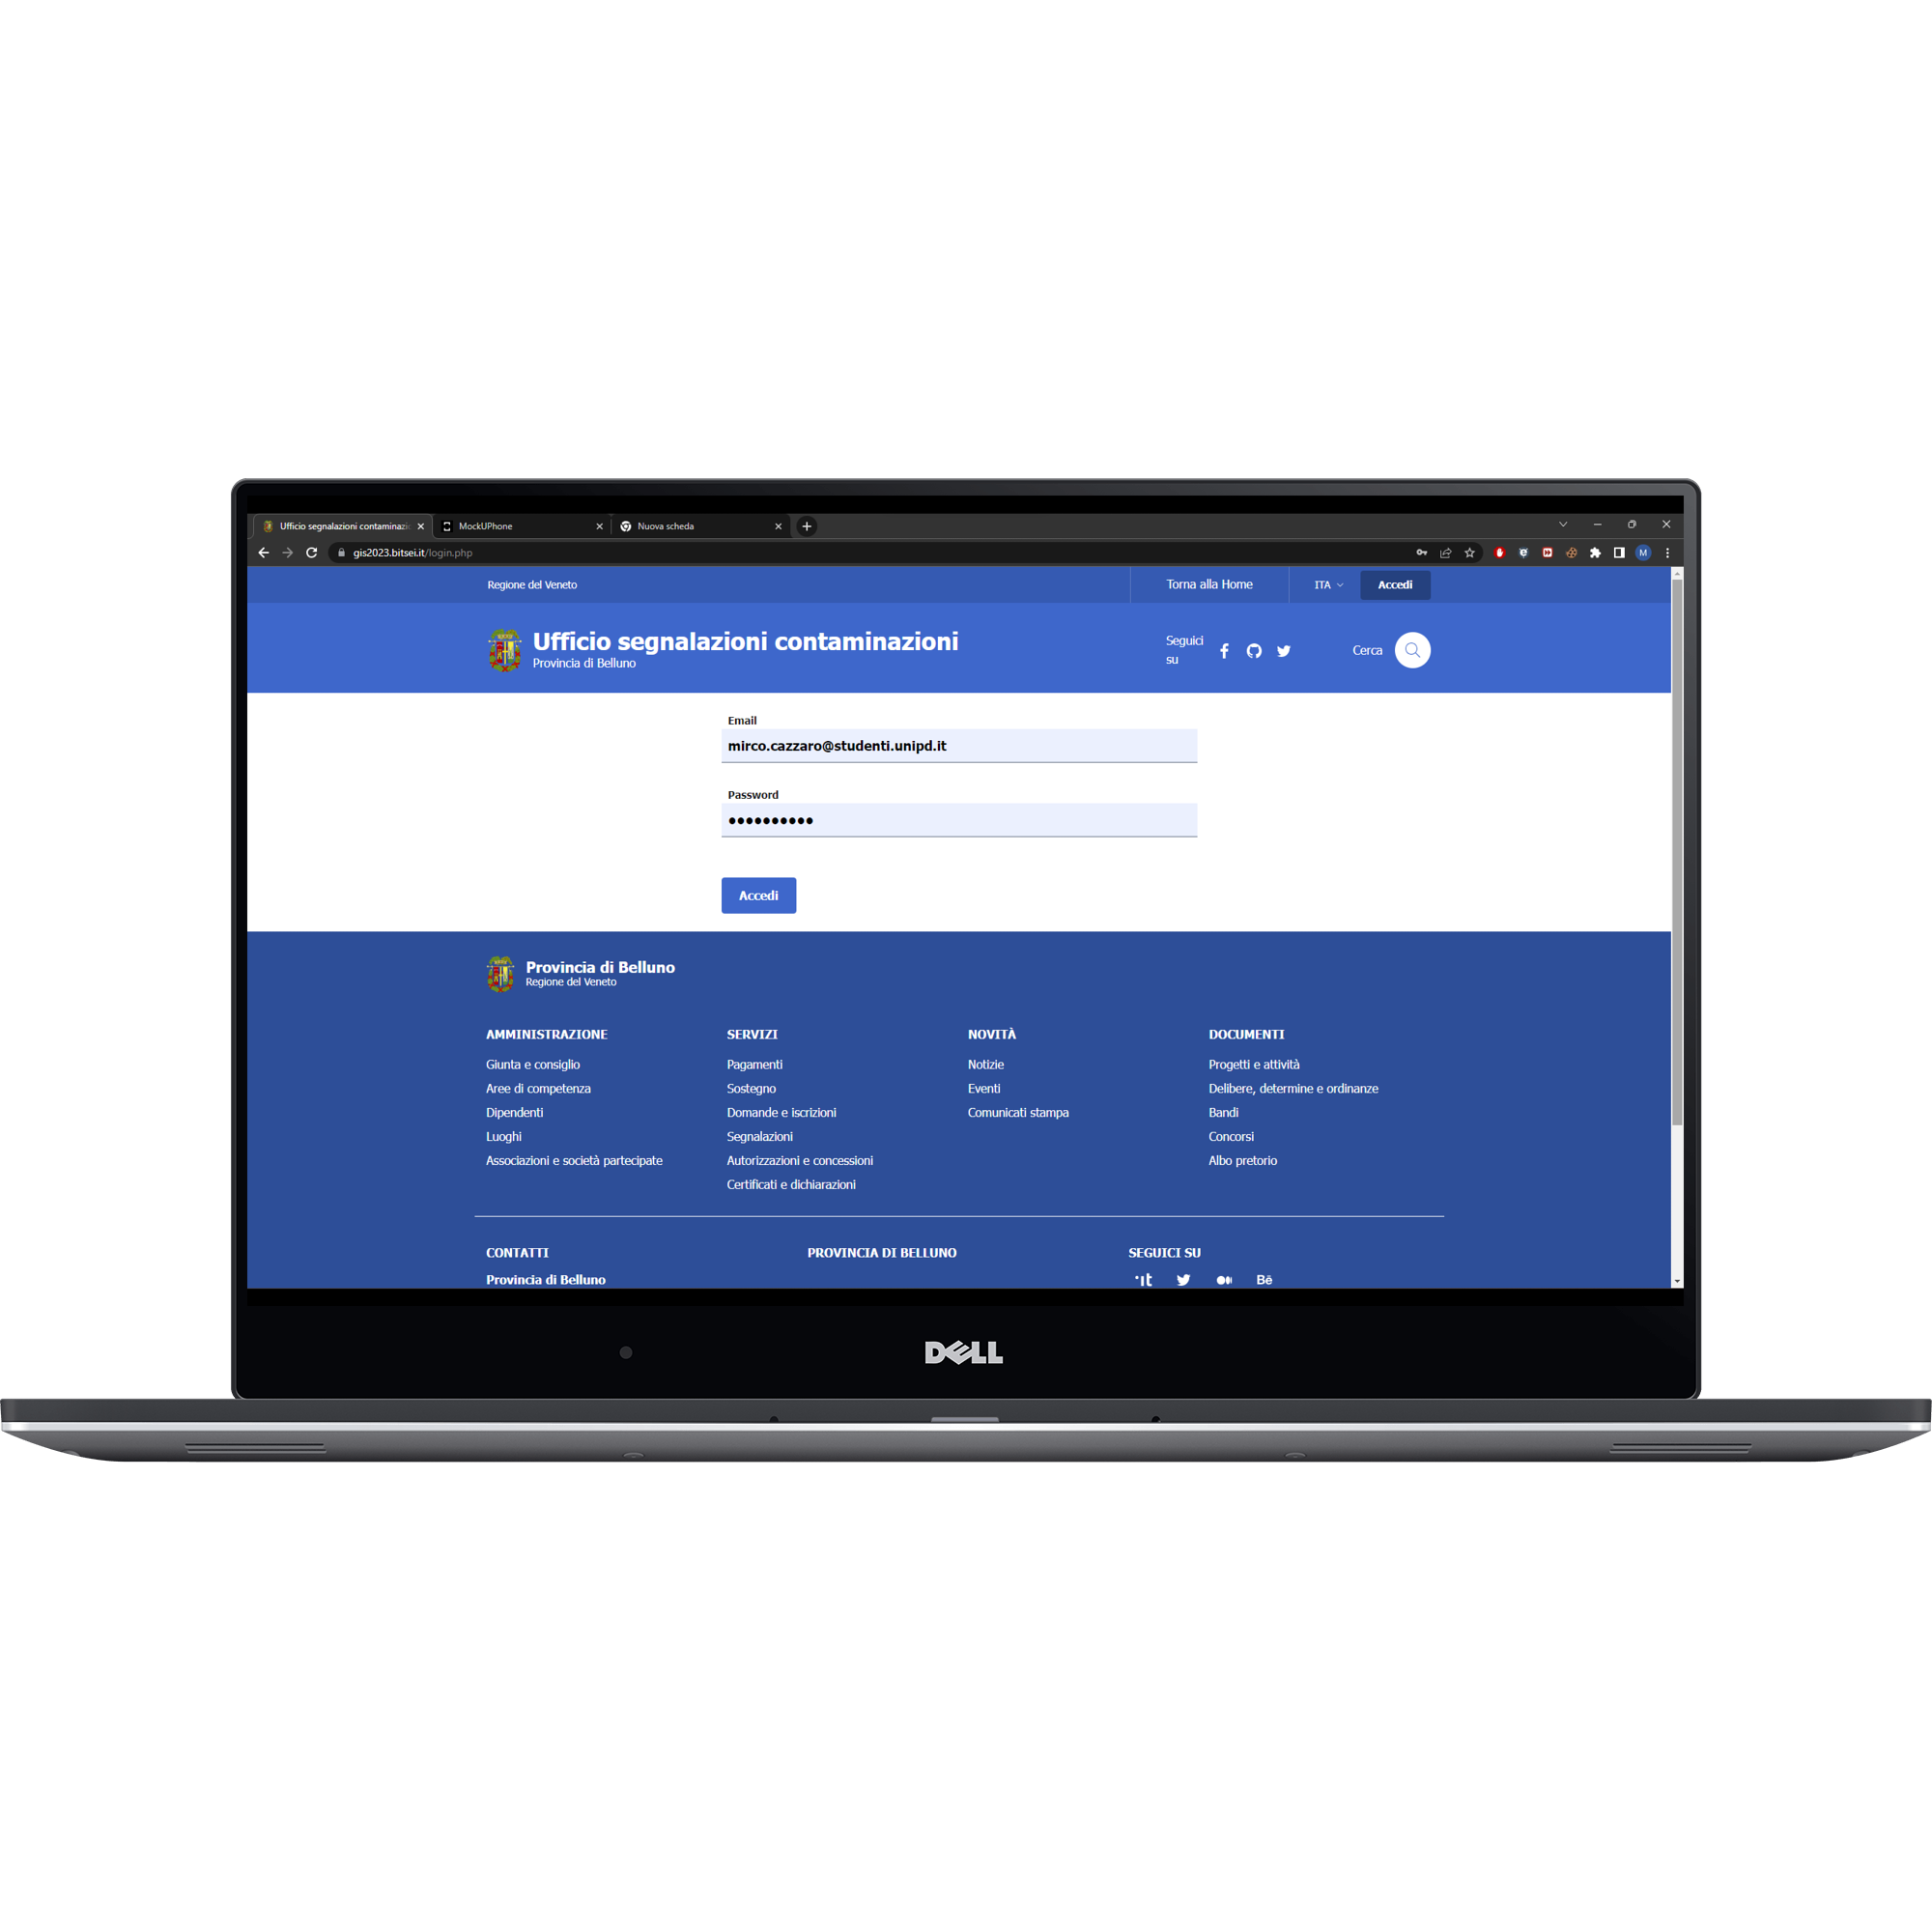
\includegraphics[width=27em]{img/login.png} \caption{Login page} \label{login} \end{figure}
    By pressing the button \textit{Accedi} on the top bar Fig[\ref{login}], we can access to the backend area reserved for the provincial technicians.
    If the login is successful a session is istantiated for the user, and he is redirected to a page that lists all the reports inserted by the citizens, filtered by year Fig[\ref{backendListing}].
    \begin{figure}[H] \centering 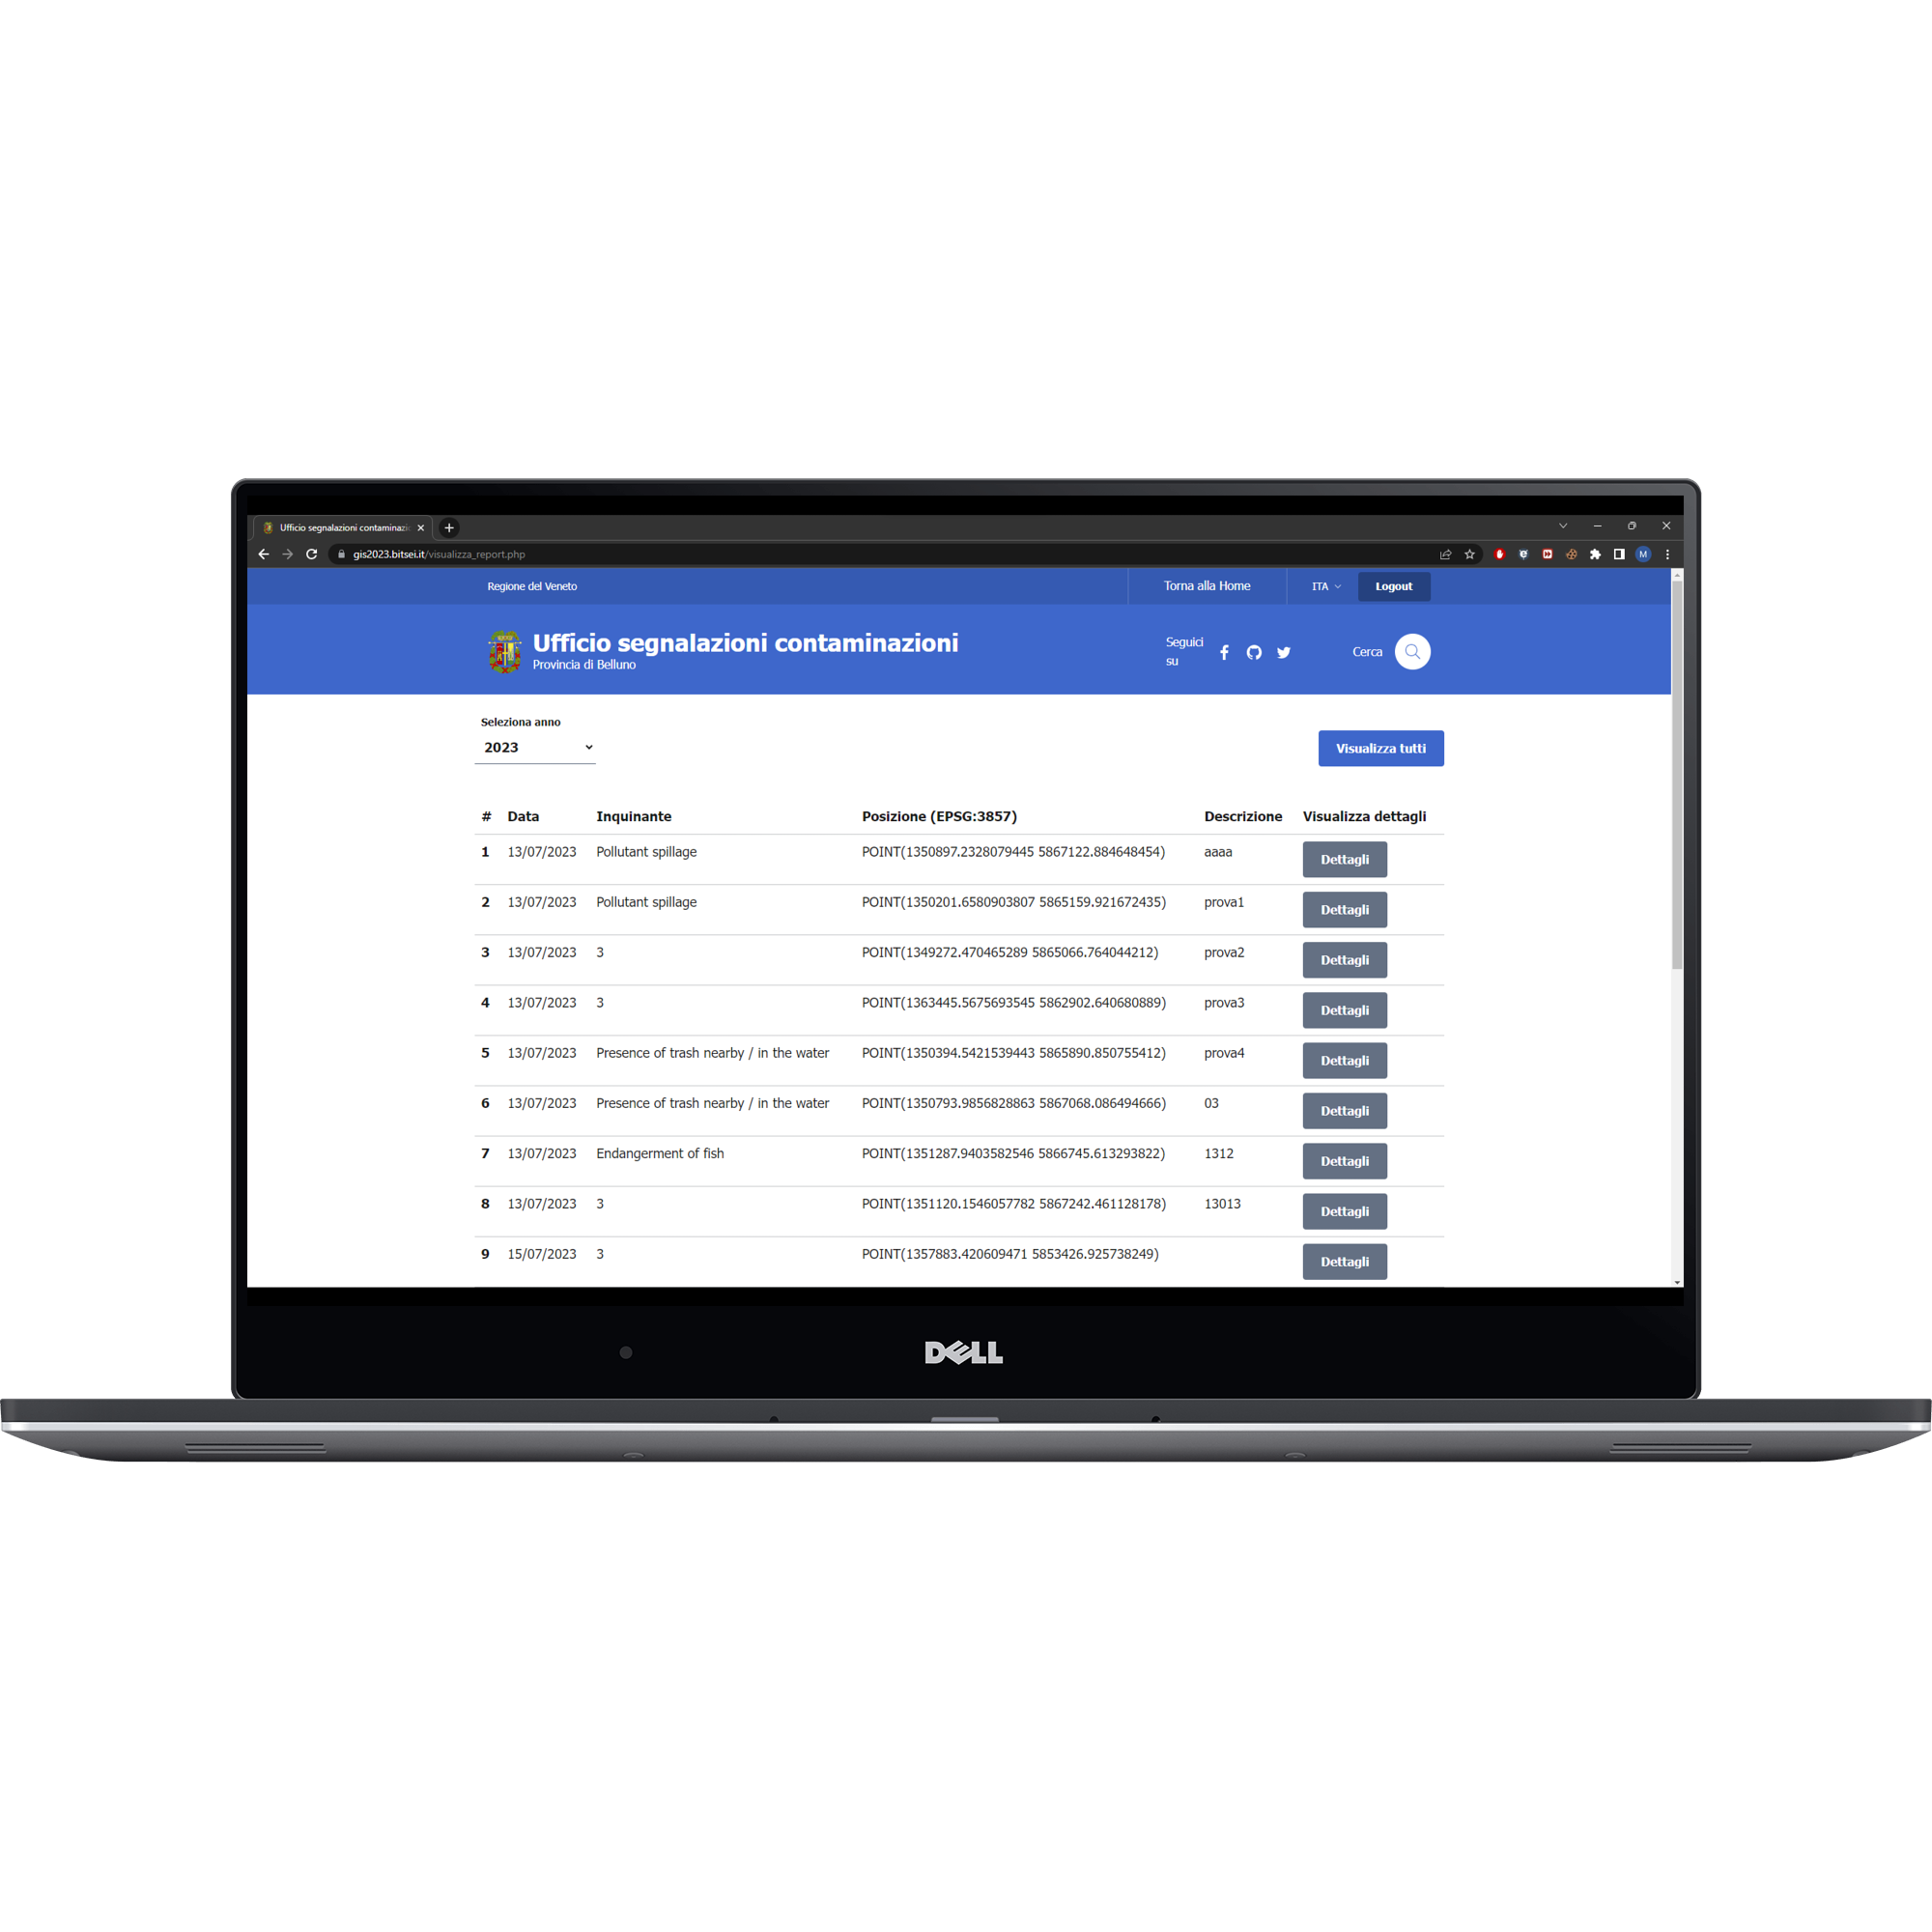
\includegraphics[width=27em]{img/home_back.png} \caption{Backend report listing} \label{backendListing}\end{figure}
    From here, an endpoint showing a series of details is available for each report Fig[\ref{reportView}]:
    \begin{enumerate}
        \item the position;
        \item the pollutant selected;
        \item the date of the report;
        \item the optional description;
        \item the optional photo;
        \item the elevation from the level of the sea of the position.
    \end{enumerate}
    \begin{figure}[H] \centering 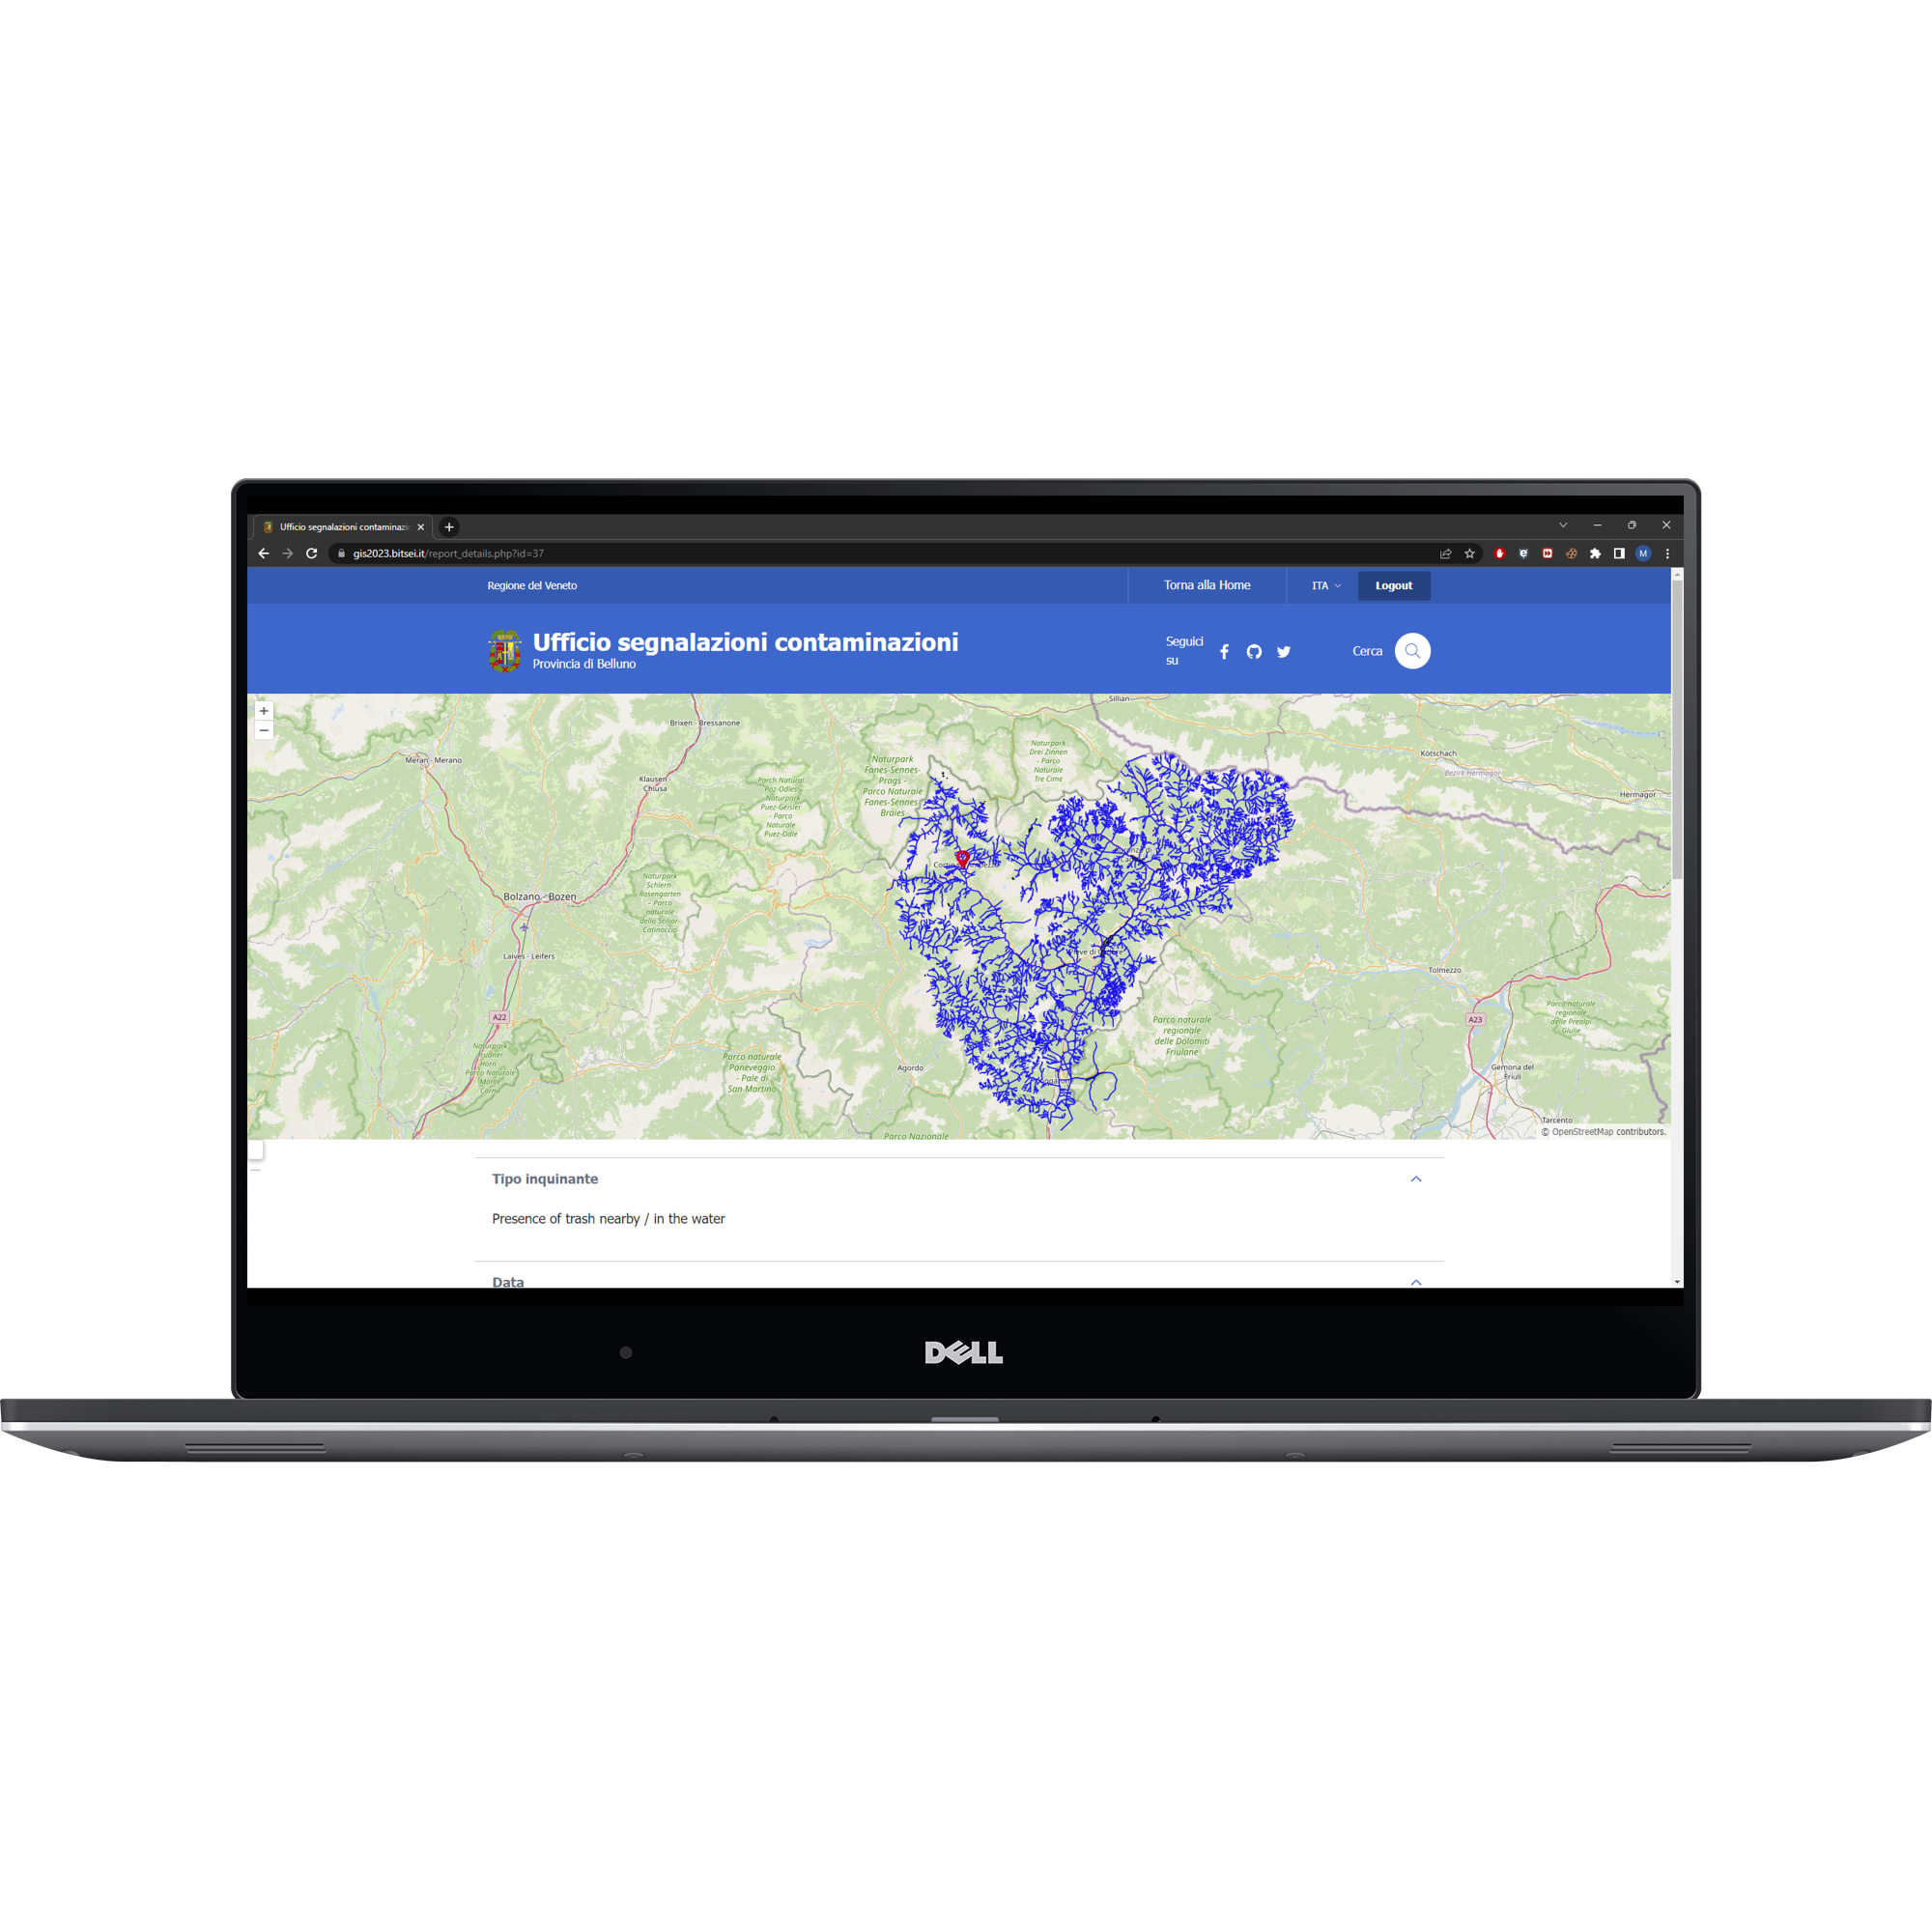
\includegraphics[width=27em]{img/pos_rep.png} 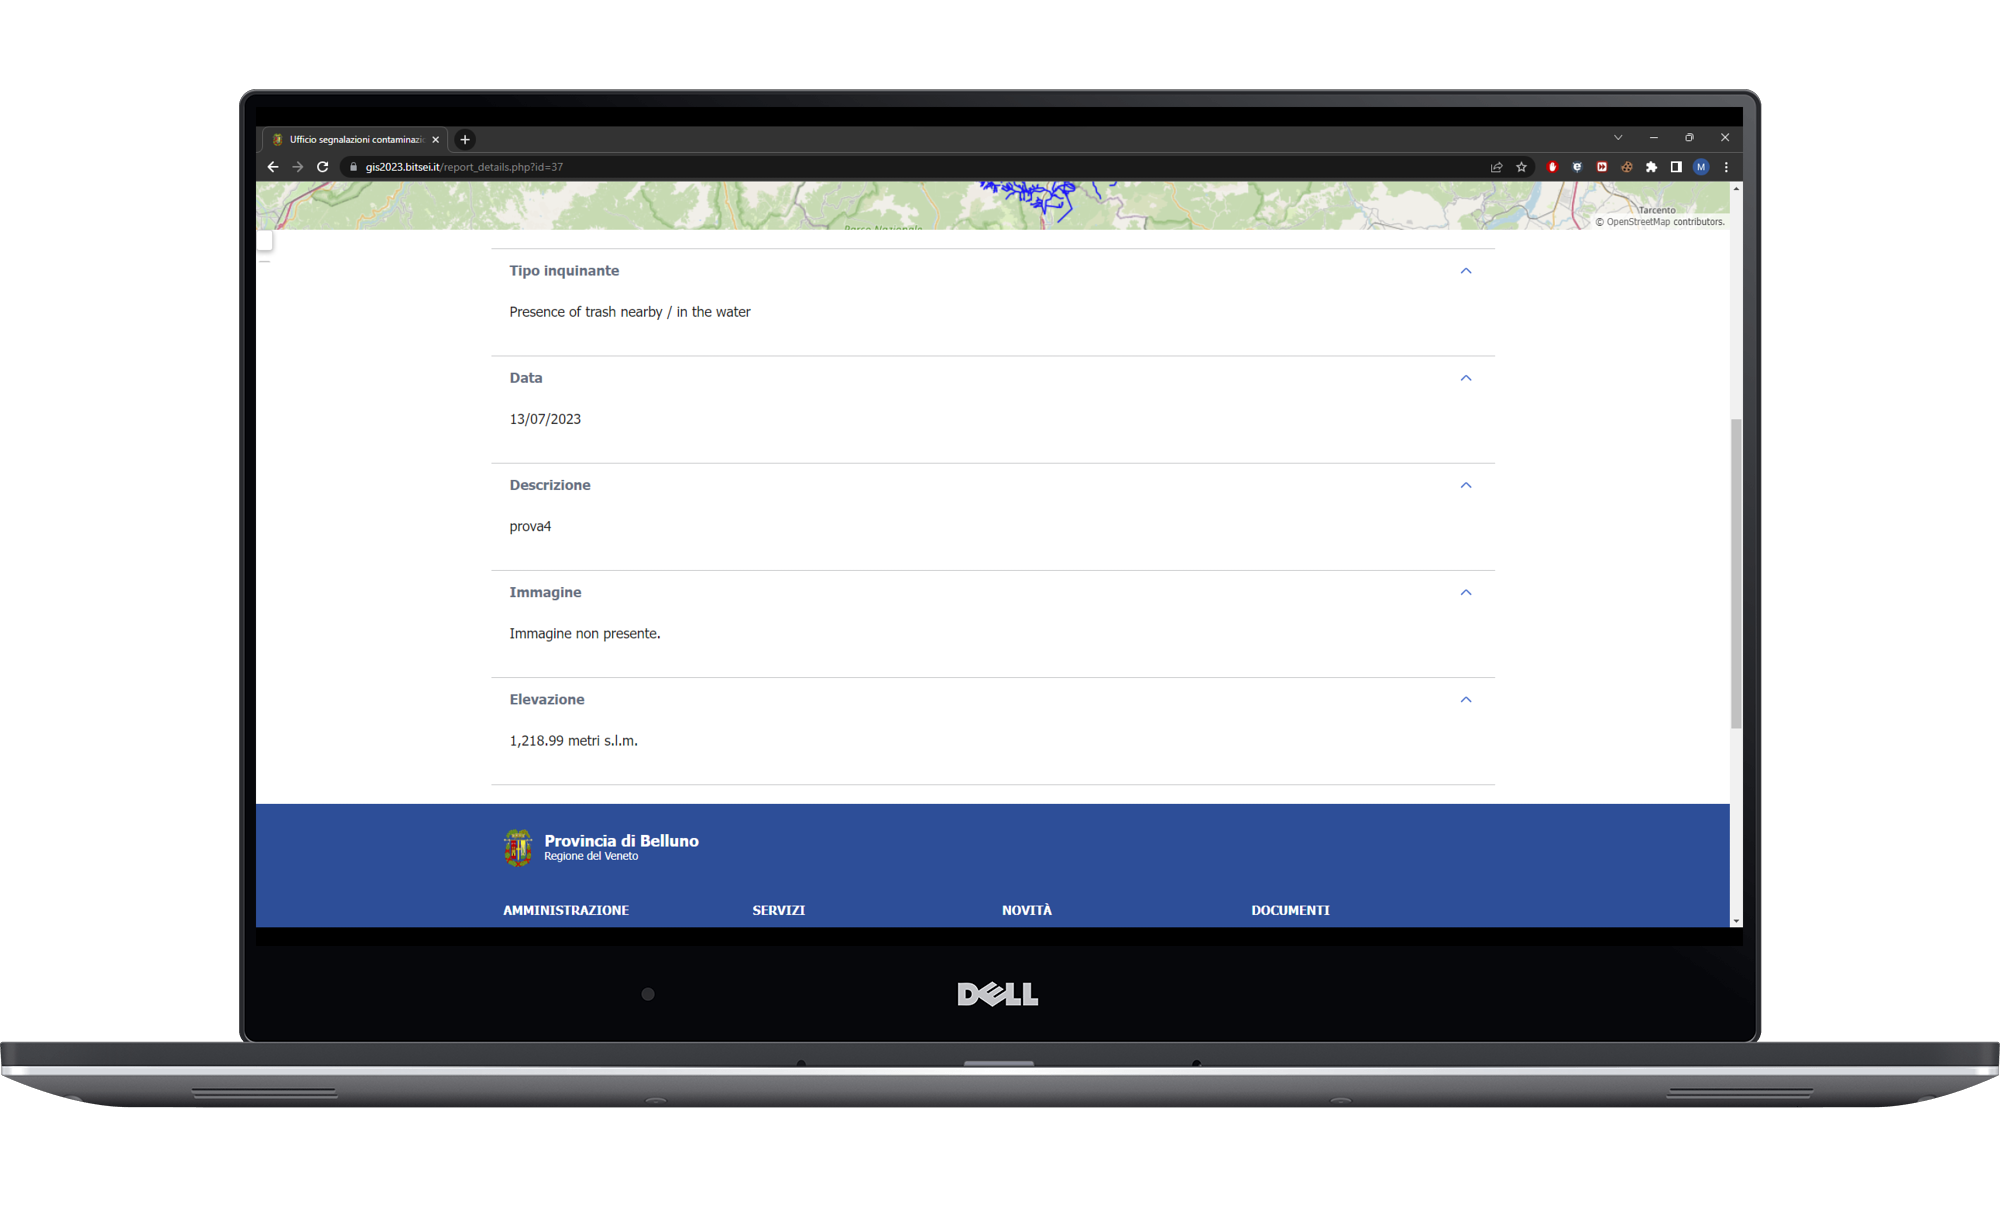
\includegraphics[width=27em]{img/dati_rep.png} \caption{View of report info}  \label{reportView} \end{figure}
    Finally, a summary map that displays the position of all the reports, with the possibility of filtering by year is available by the button in the home page \textit{Visualizza tutti} Fig:[\ref{allPositions}].
    \begin{figure}[H]\centering 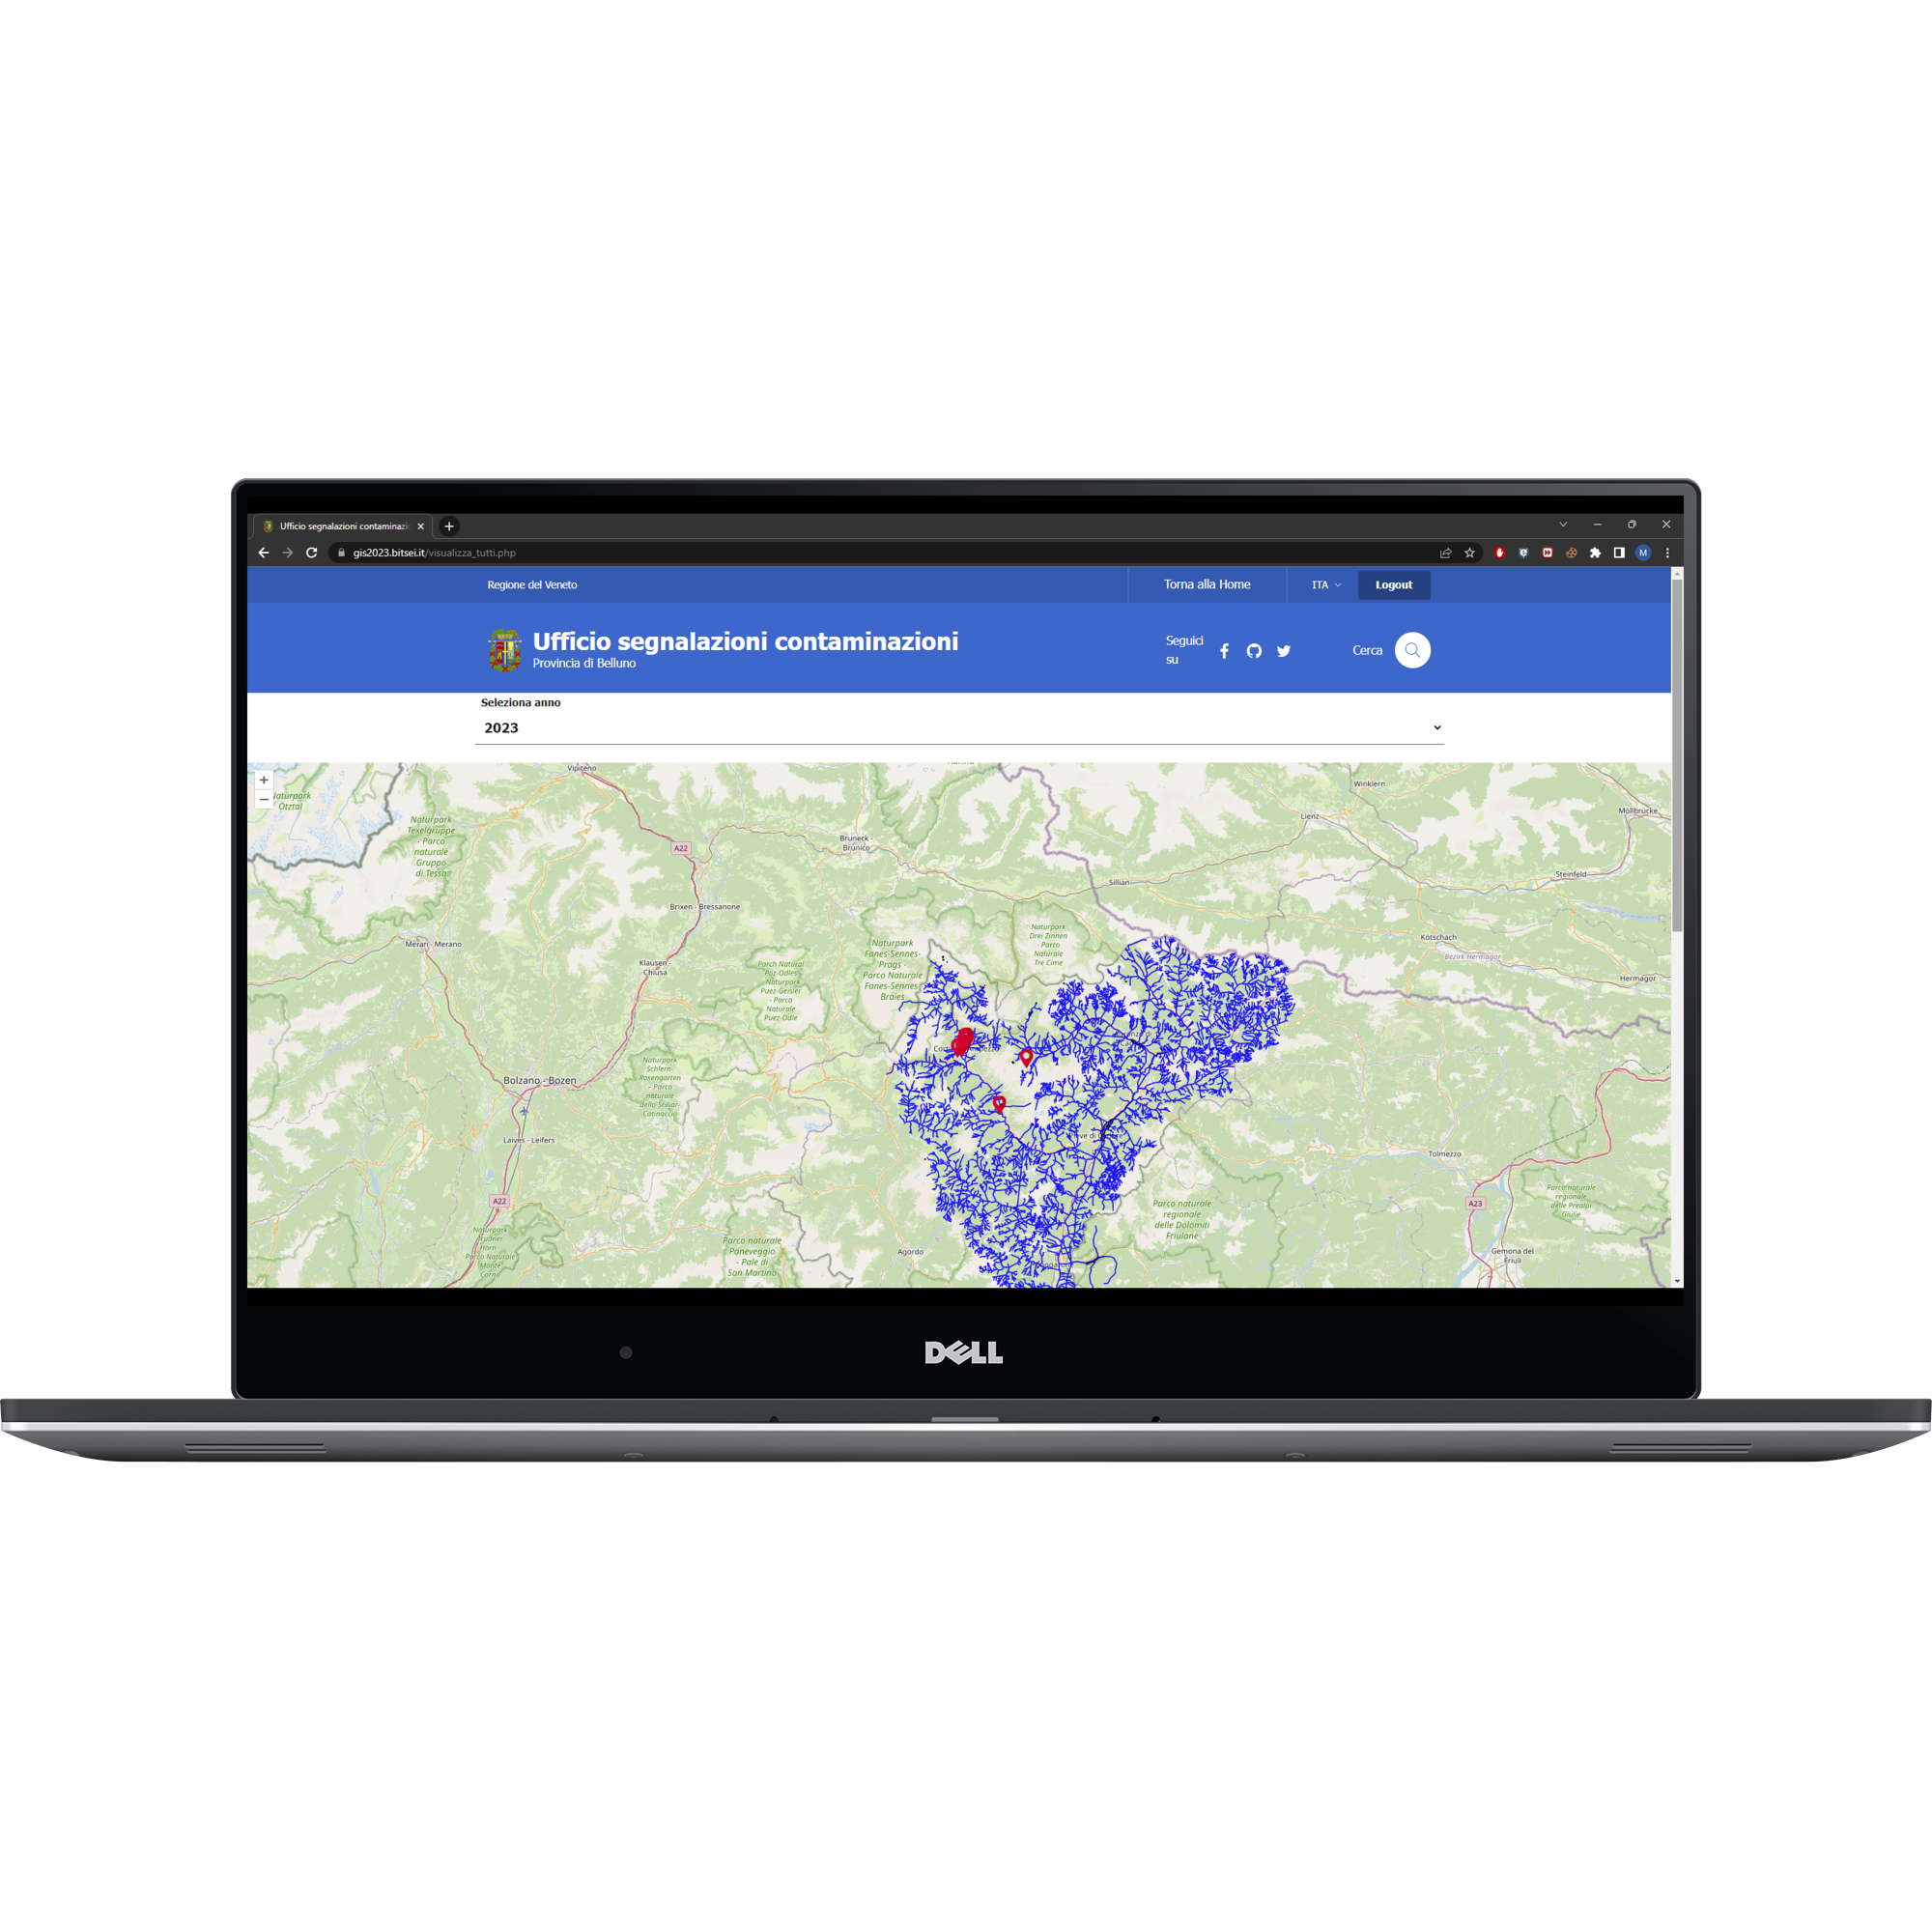
\includegraphics[width=27em]{img/all_reports.png} \caption{View of all report positions} \label{allPositions}\end{figure}
    
\end{itemize}

\subsubsection{OpenJUMP plugin}
The plugin is mainly implemented by 3 classes their functionalities are:

\begin{itemize}
    \item \textit{Plugin.java} Is the main class, it establish the plugin, and it finds the first nearest 3 monitor units and all reports in a 500m range.
    \item \textit{Login.java} By using javaSwing it enables the user for making a login to the database.
    \item \textit{Database.java} It connetes the plugin to the database, it can retrive all the monitor units and report stored.
\end{itemize}

For more tecnical infrmation the projact has a javadoc.

\begin{figure}[H]
    \centering
    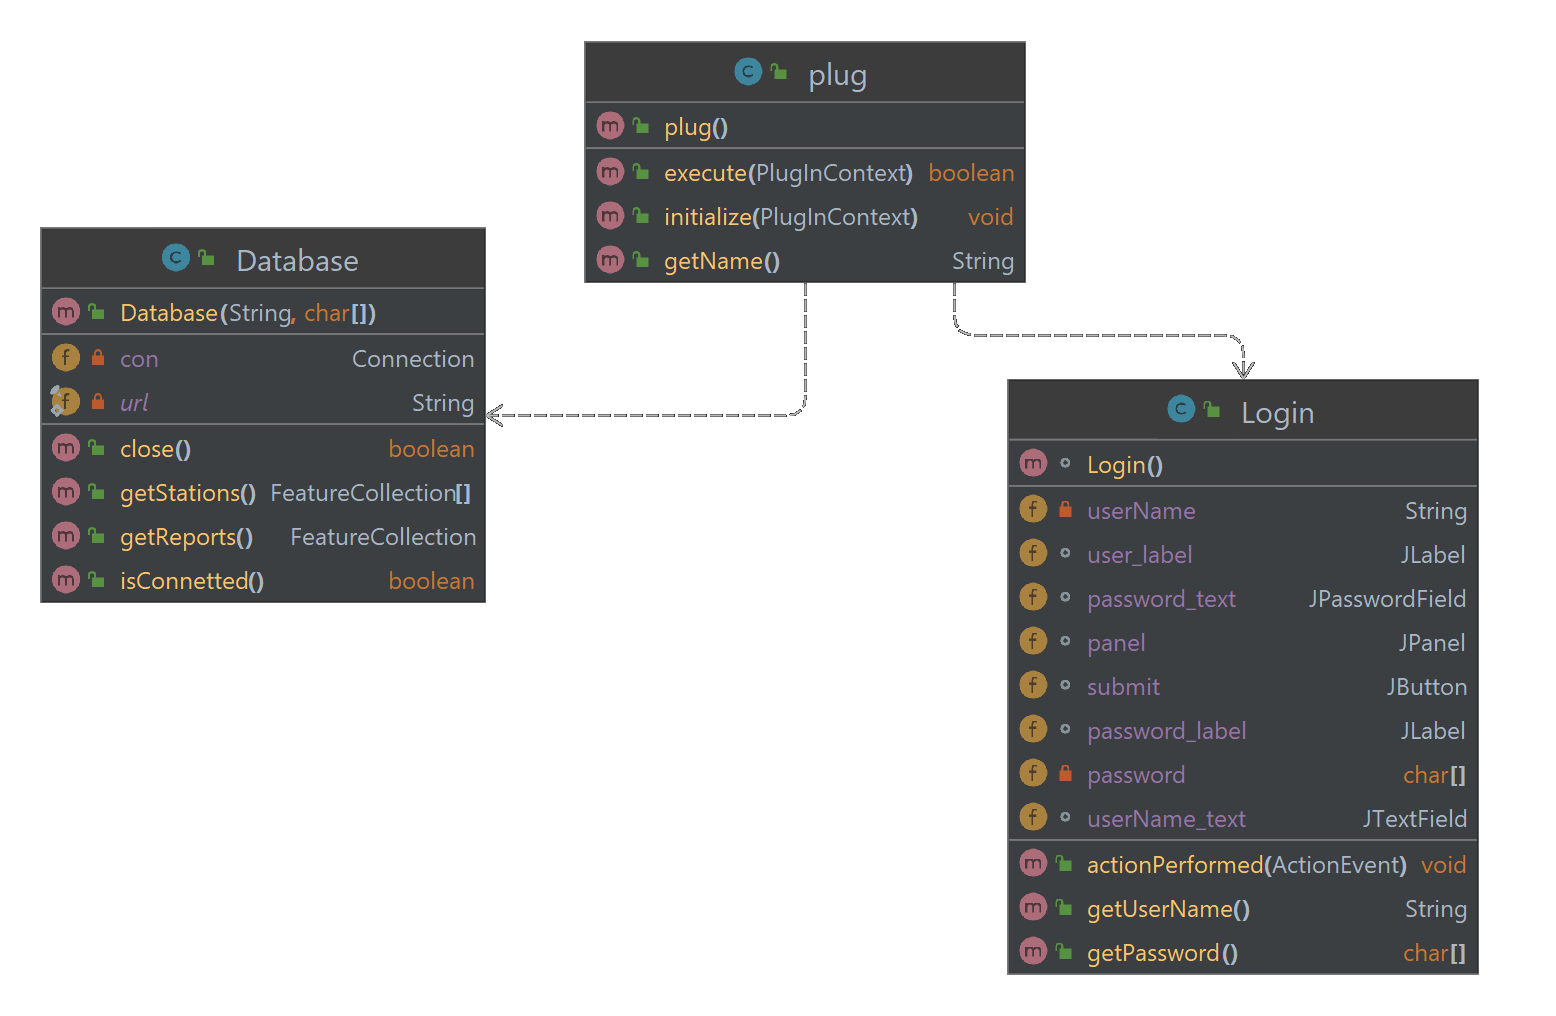
\includegraphics[width=25em]{img/classdiagram.png}
    \caption{UML diagram}
    \label{uml}
\end{figure}

Differently from the webapp, here a specific initial configuration on the user's terminals needs to be setted up.
This kind of initial support is by the way provided by our company and so no tutorial needs to be included in this document. \\
As specified we will use OpenJUMP as GIS software, the open source nature of OpenJUMP grants us the full acessibilty of it's interfacess for 2D geometry manipulation.
The Output layers will be located in the "Result" folder. All the relevant data inside the database will be loaded in OpenJUMP so the tecnichian can see all the informations about reports and monitor units.
The plugin will work as the following:

\begin{enumerate}
    \item The user will launch the plugin.
    \item The plugin will ask for the credentials for database connection fig:[\ref{optuTorial1}]. 
    \begin{figure}[H]
        \centering
        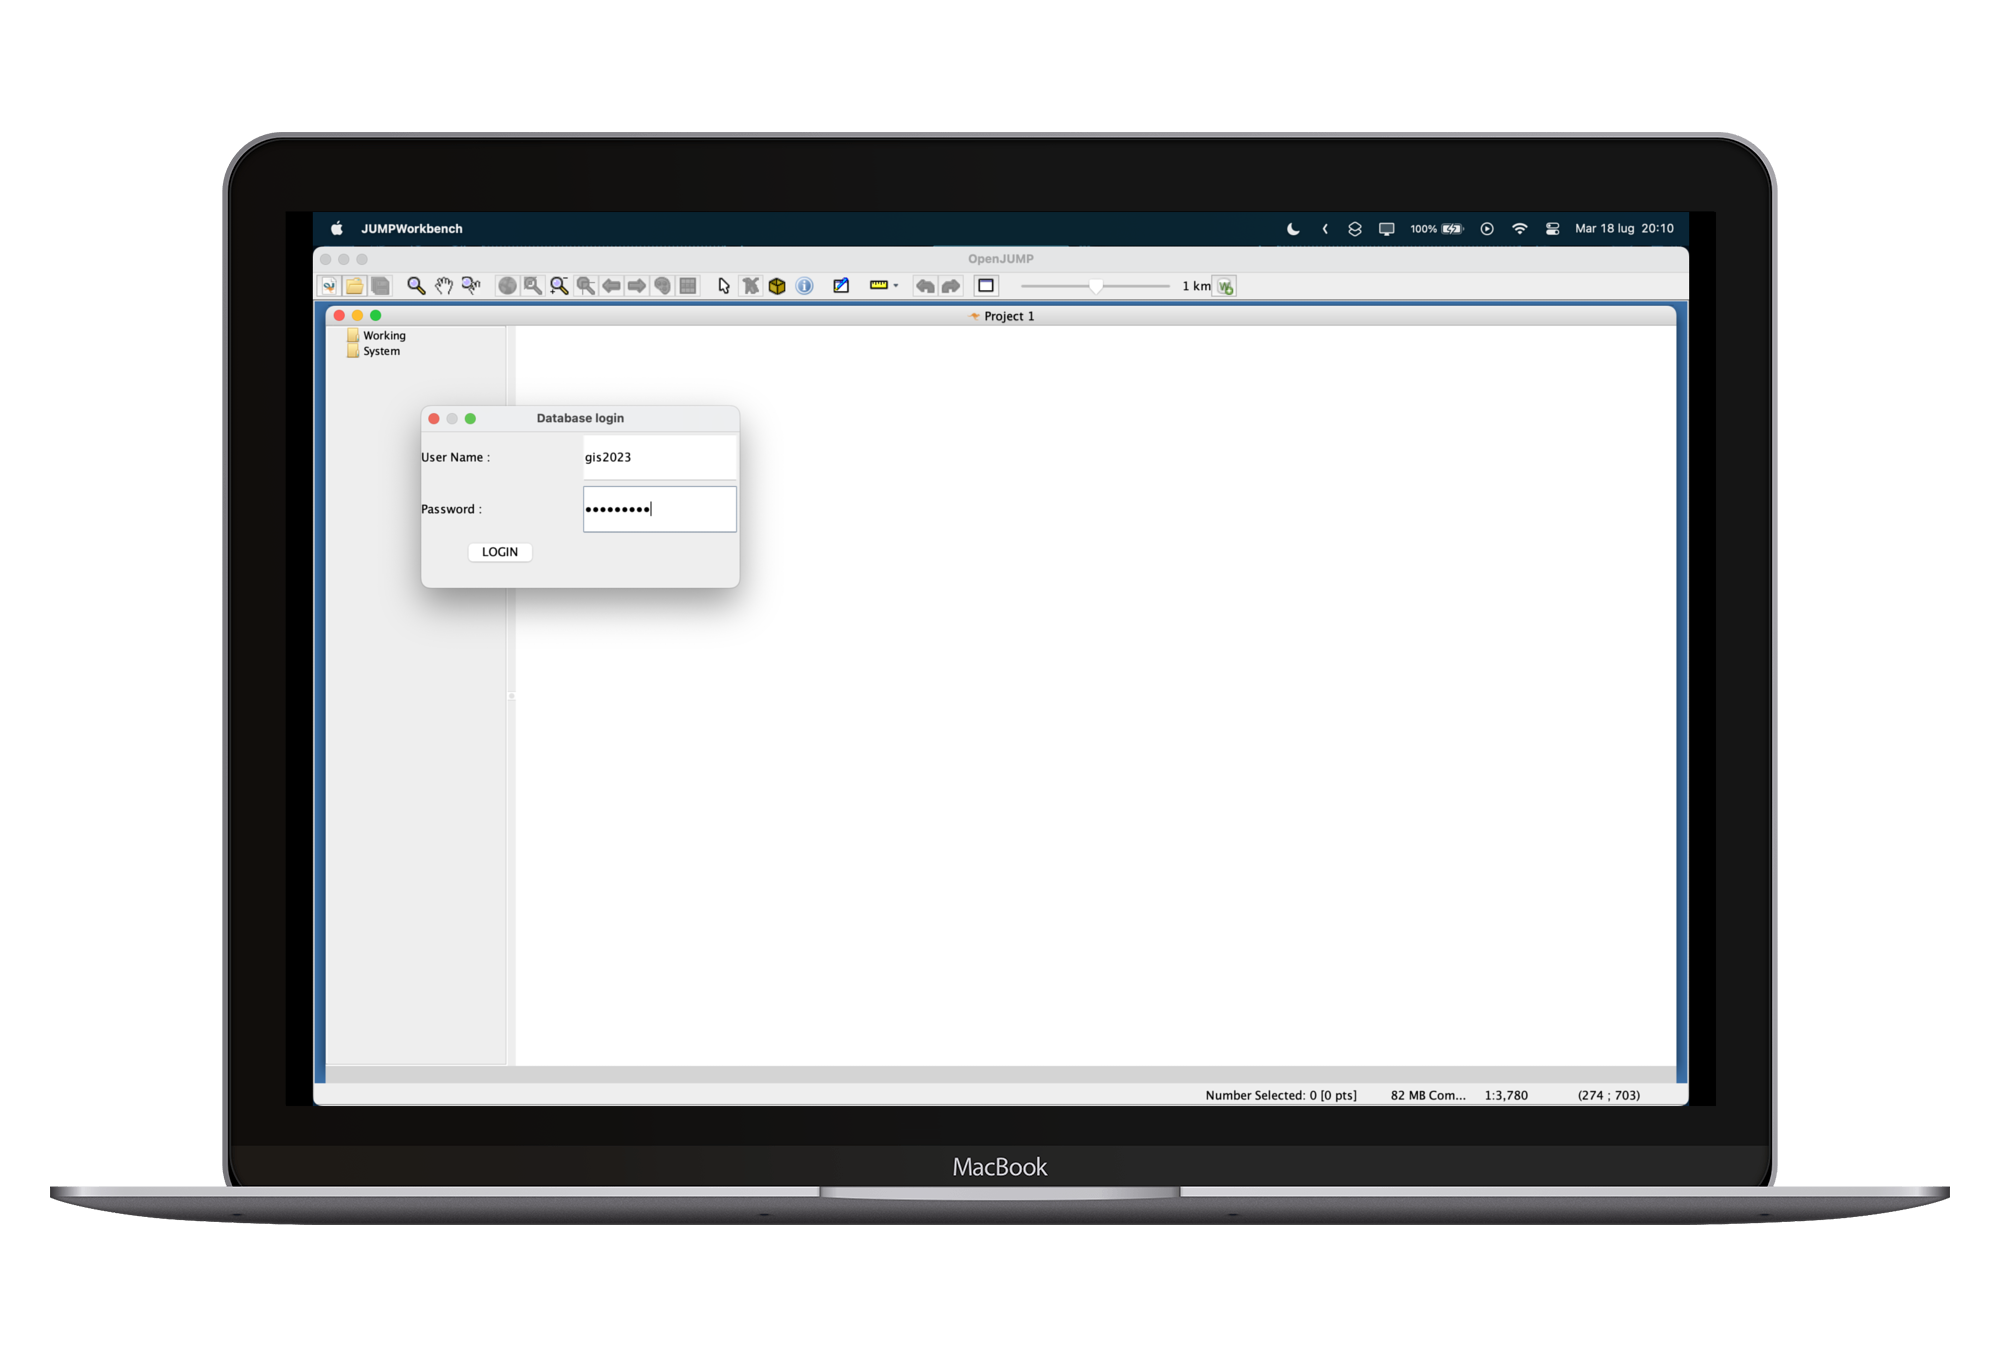
\includegraphics[width=27em]{img/op1.png} \caption{Database login} \label{optuTorial1}
    \end{figure}
    \item The plugin will load the layers of the reports and monitor units.
    \item The user will choose the report to visualize fig:[\ref{optuTorial2}].
    \begin{figure}[H]
        \centering
        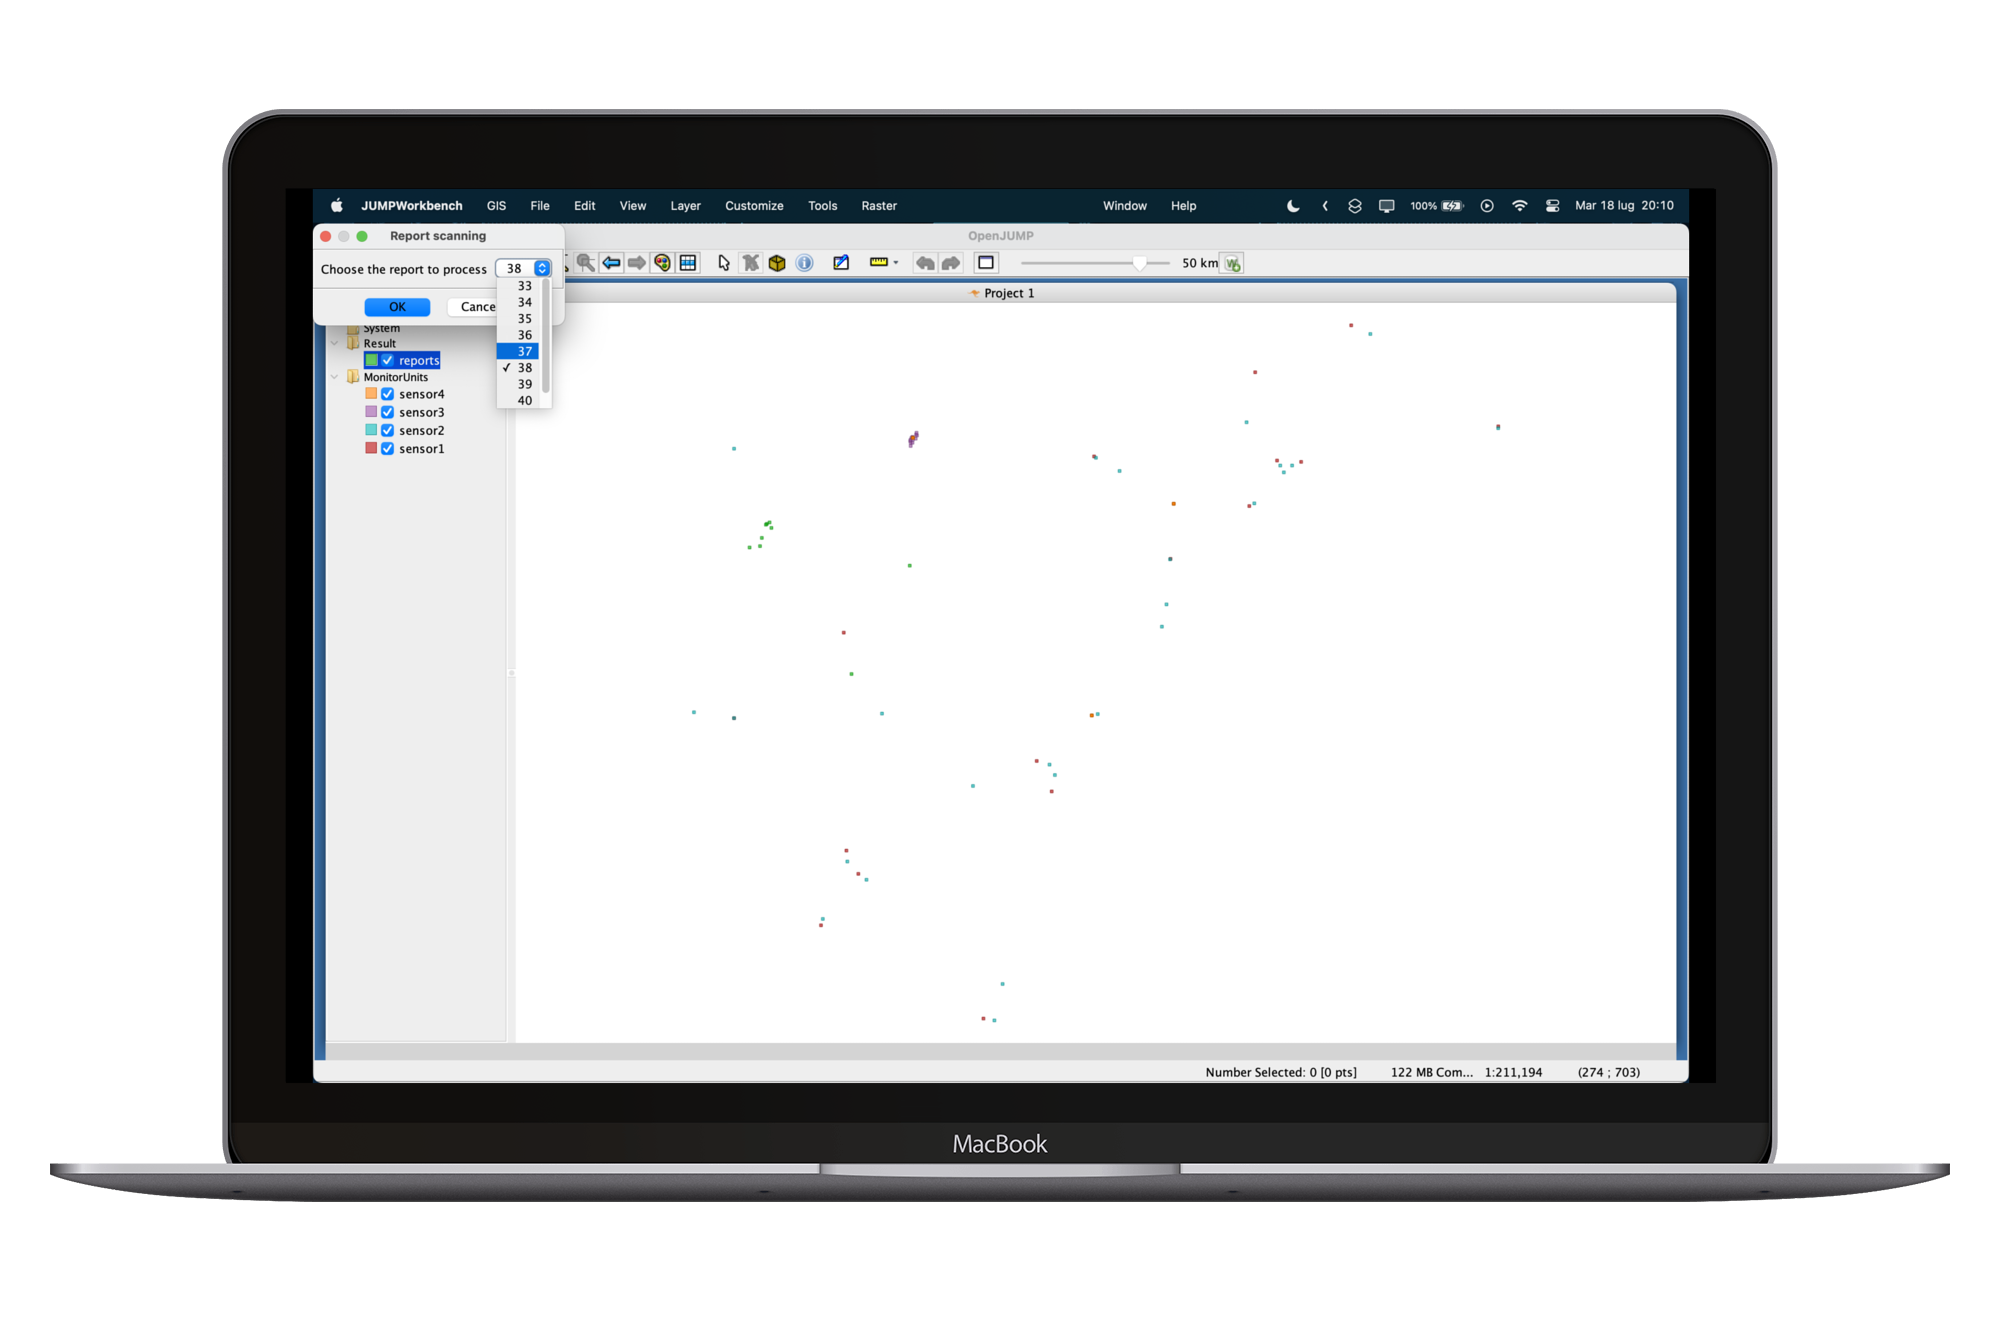
\includegraphics[width=27em]{img/op2.png} \caption{Report selection} \label{optuTorial2}
    \end{figure}

    \item The plugin will find the closest three monitor units to the report position (two upstream one downstream) and they will be linked to the position of the report chosen fig:[\ref{optuTorial3}].
    \begin{figure}[H]
        \centering
        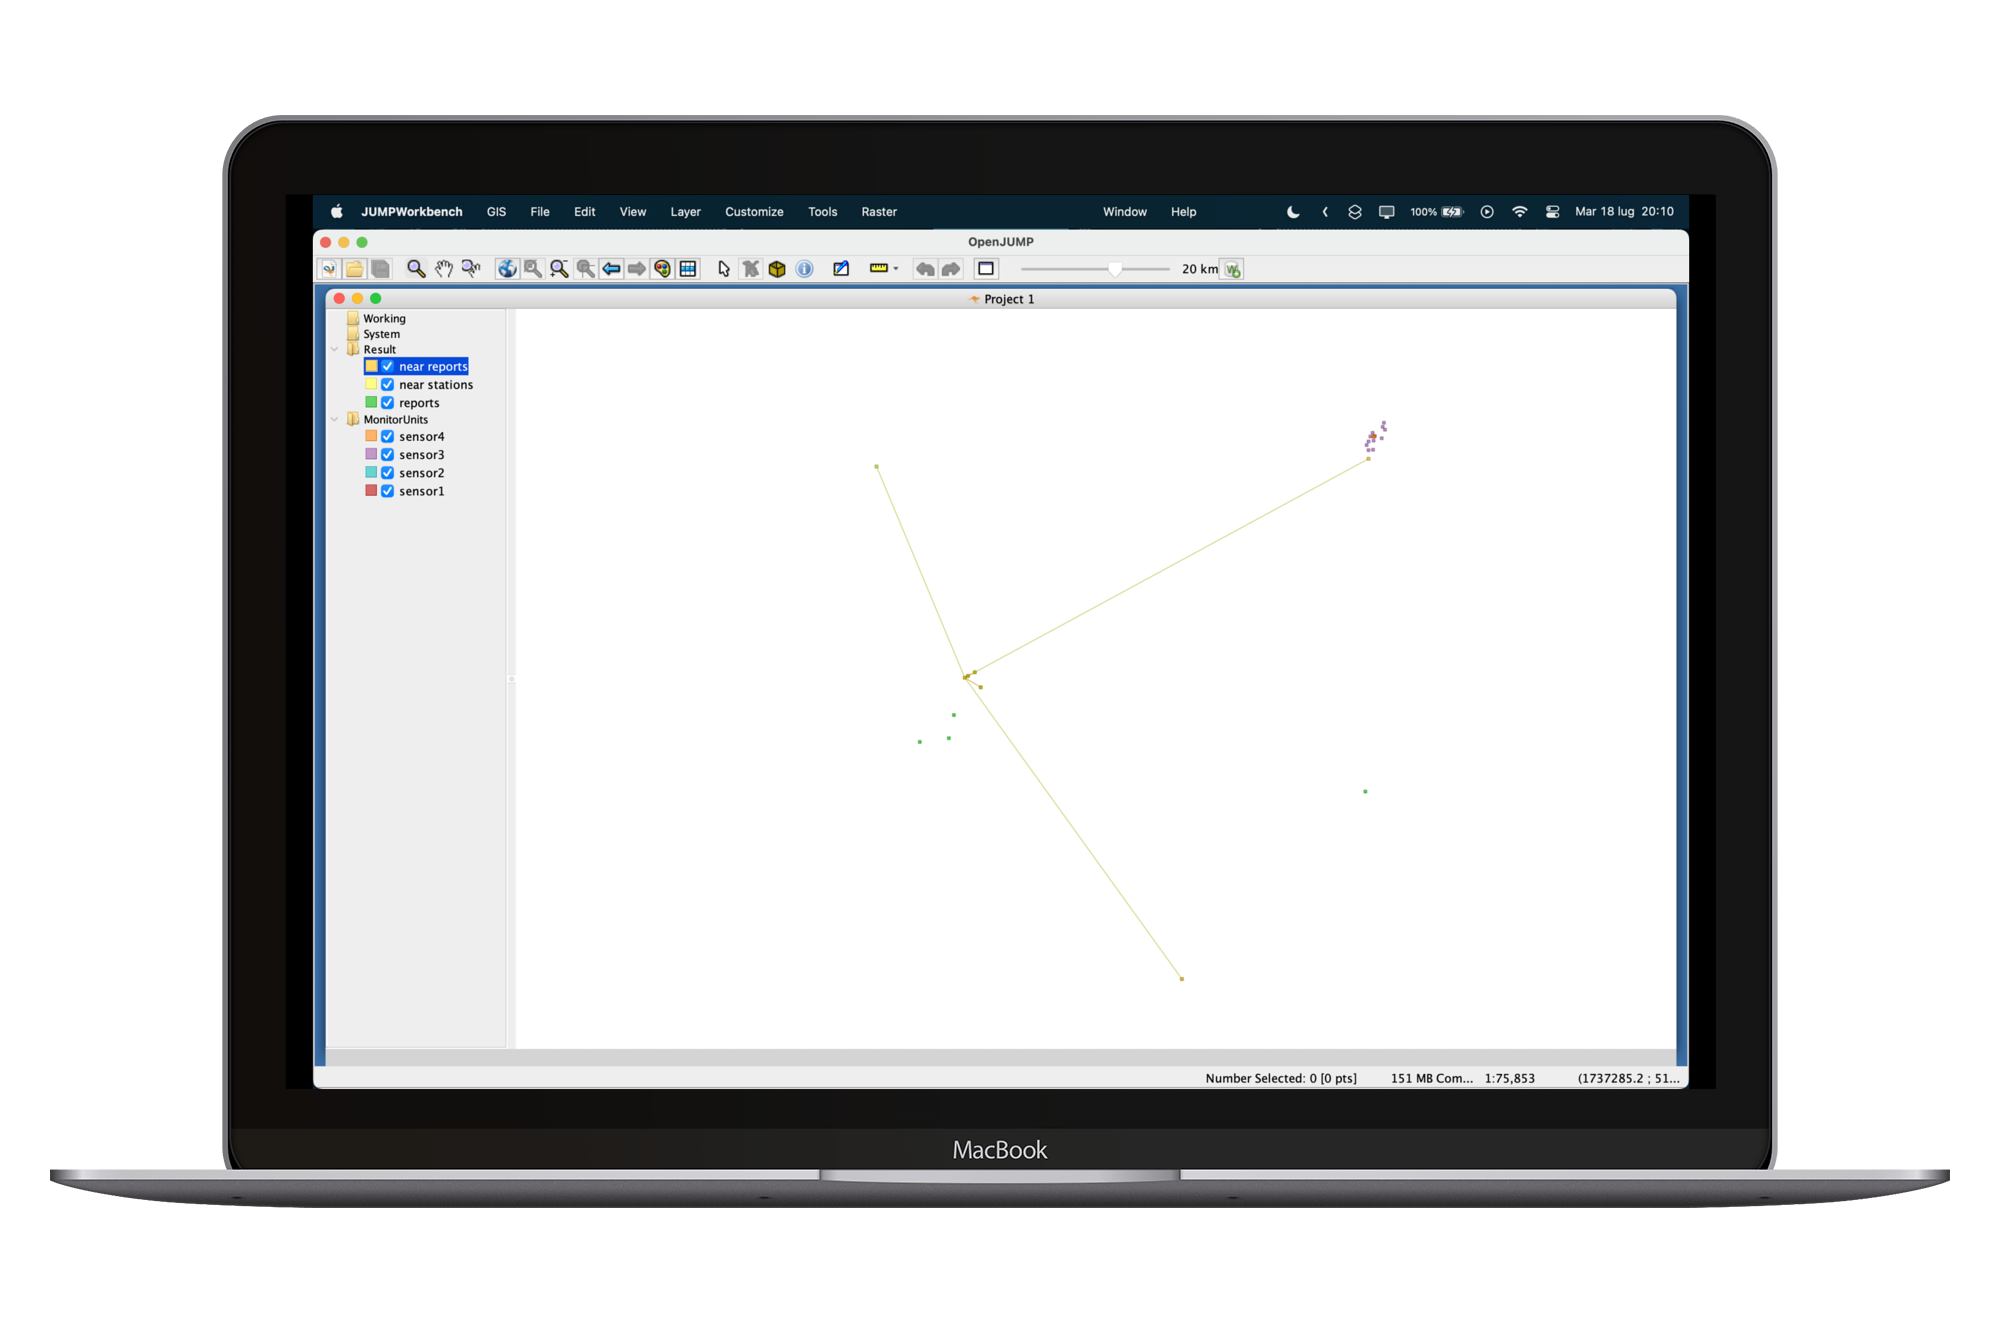
\includegraphics[width=27em]{img/op3.png} \caption{Report connetions} \label{optuTorial3}
    \end{figure}

    \item The plugin will find all the reports in a range of 500 meters and they will be linked to the report chosen.
\end{enumerate}



\subsection{Other features not implemented}

For the final delibery the project shold have this other features not implemted:

\begin{itemize}
    \item an interface for the 3 technicians that allows them to modify, remove or add the intakes of the various companies, every tecnichian will have it's own account for managing it.
    \item an interface for thetechnicians which allows them to check the maintenance scheduling and indicate when it was done, it can displaye the history of all the maintenance already carried out.
    \item a program that reads the data from the 10 gateways and writes the data to the database.
    \item a danger ranking for the report generated by an AI powered technologies, by using Natural Language Processing (NPL) and Computer Vision techniques the AI will score a ranking in the range 0 to 10, where 10 is very dangerous.
\end{itemize}

\subsection{Database}
\subsubsection{ER Schema}
\begin{figure}[H] \centering 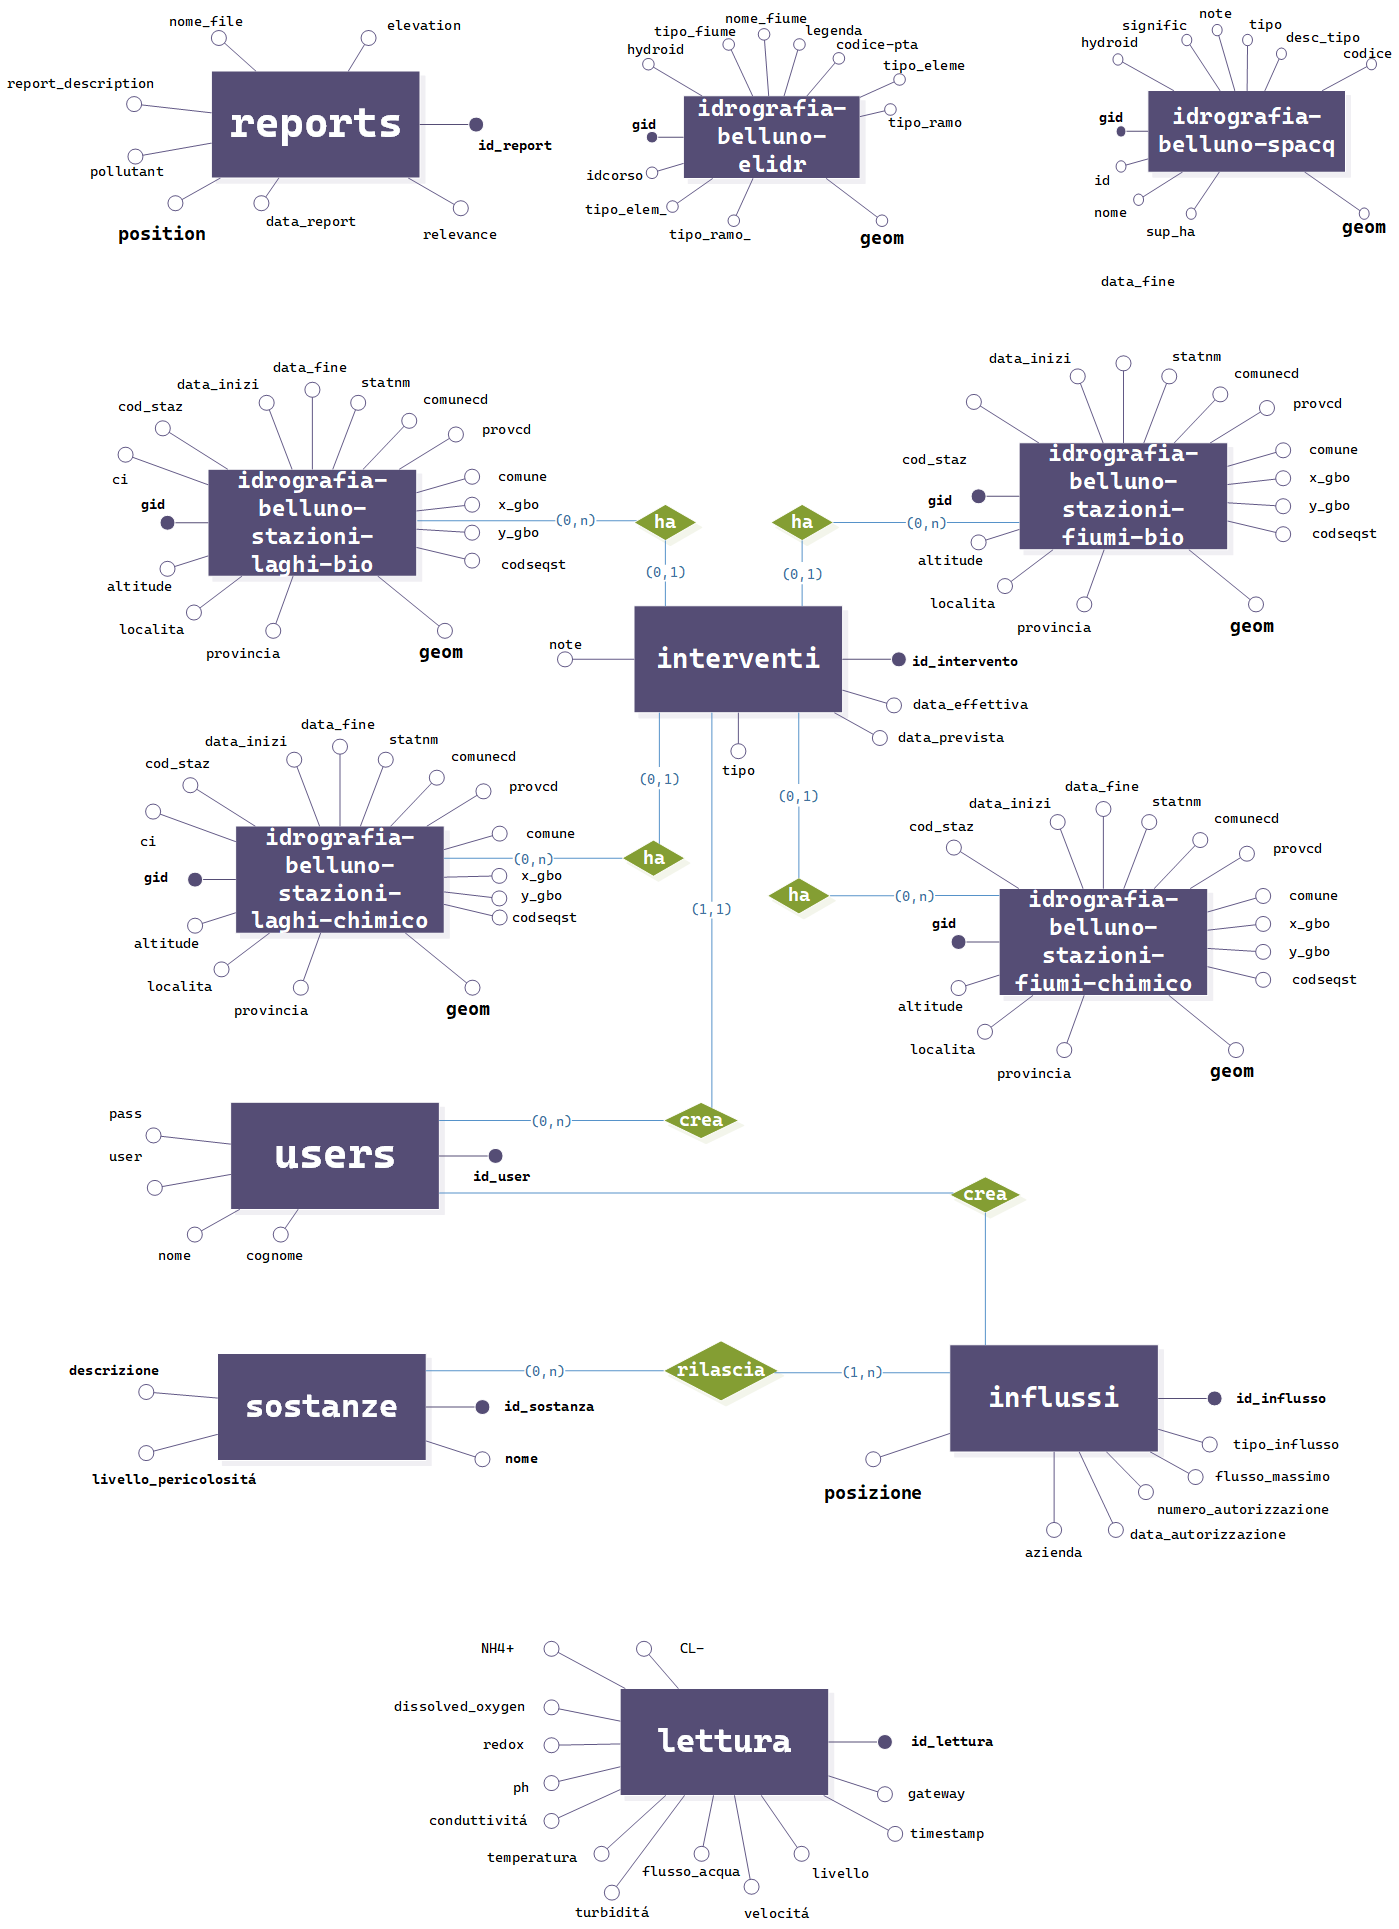
\includegraphics[width=39em]{img/ERSchema.png}  \caption{ER schema} \label{er} \end{figure}

\subsubsection{Description of entities and relationships}
As the schema displays Fig[\ref{er}], we can see that six of the entities are related to each shapefile regarding data coming from the Region of Veneto and ARPA Veneto.
For what concerns spatial data representing rivers and lakes, the entities are:
\begin{itemize}
    \item \textit{idrografia-belluno-elidr};
    \item \textit{idrografia-belluno-spacq};
\end{itemize}
The relations that are related to the 4 different typologies of monitoring units instead are:
z\begin{itemize}
    \item \textit{idrografia-belluno-stazioni-laghi-bio};
    \item \textit{idrografia-belluno-stazioni-fiumi-bio};
    \item \textit{idrografia-belluno-stazioni-laghi-chimico};
    \item \textit{idrografia-belluno-stazioni-fiumi-chimico}.
\end{itemize}
As it is visible from the schema, these entities are in relation with the entity \textit{interventi}. This entity represents a maintenance event made by one technincian phisically on a monitoring unit. Due to the limitation of the E-R representation, another constraint need to be exploited: each record in \textit{interventi} has at least and at most one foreign key relation with one record in one of the four stations entities.
An \textit{intervento} is made by one connected \textit{user}: this entity holds data and credentials of each user (technicians and employees) of the provincial office. \\
As a technician user is in charge of making an \textit{intervento}, an employee of the provincial office is in charge (between all) of managing the insertion and the deletion of intakes into rivers and lakes. Intakes are represented by the \textit{influssi} entity, with all the data necessary to represent them. Since a company can release from an intake many different substances, the representation of them in an dedicated entity was necessary: this imply that employee will need to insert, delete or update polluting substances (\textit{sostanze}) separately. \\

Lastly, two important but not relationed entities are in the database:
\begin{itemize}
    \item \textit{reports}: this entity records all the reports made by the citizens. Between all the field, a \textit{relevance} field that as explain before is set to allow future installation of an external software (based on AI technologies) that will be able to assign a relevance score to each report.
    \item \textit{letture}: this entity records the data read from the ten public web gateways that collect the information from the 90 monitoring units. The recording operation of this data is necessary because of the historicization and interrogation requirement.
\end{itemize}

\subsubsection{Data volumes}
The last two described entities (\textit{reports} and \textit{letture}), differently from the others, can require a lot of disk space on the system server.
A specific analysis of space needed for the reports cannot be exact and neither estimated until we do not have some statistics on the popularity of the system among the citizens: an approach can be to allocate a quite big amount of space initially and to observe the usage in the first months after the installation of the system, so to reduce or increase it. \\
For the \textit{letture} entity is instead possible a more precise estimation: since a separated script in charge of periodically read data from the web gateways and write them on the database will be set up, by knowing the reading frequency (assuming in seconds) of the monitoring units, and assuming an history of one year in the database, the space required from this entity will possibly be: \\
\begin{figure}[H]
    \centering
    \begin{math}
        Space = 60\cdot\frac{86400}{Frequency}\cdot365\cdot90
    \end{math}
    \caption{Approximation of the size of the \textit{readings} table in 1 year.}
    \label{letture_space}
\end{figure}
Where \textit{60} is our estimation in byte of the size of a record, \(\frac{86400}{Frequency}\) is the number of readings per day and \textit{90} is the number of monitoring units [\ref{letture_space}].
   
\subsubsection{Final considerations}
It is important to keep in mind that even if many relations seem to be missing (i.e. an intake is not linked to the corresponding river nor lake, etc.), a topological database like this can rely on the implicit spatial relations that can be detected in the logic of the application by using topological libraries (i.e. \textit{JTS}) or directly using \textit{PostGIS} functions.


